% Options for packages loaded elsewhere
% Options for packages loaded elsewhere
\PassOptionsToPackage{unicode}{hyperref}
\PassOptionsToPackage{hyphens}{url}
\PassOptionsToPackage{dvipsnames,svgnames,x11names}{xcolor}
%
\documentclass[
]{article}
\usepackage{xcolor}
\usepackage{amsmath,amssymb}
\setcounter{secnumdepth}{5}
\usepackage{iftex}
\ifPDFTeX
  \usepackage[T1]{fontenc}
  \usepackage[utf8]{inputenc}
  \usepackage{textcomp} % provide euro and other symbols
\else % if luatex or xetex
  \usepackage{unicode-math} % this also loads fontspec
  \defaultfontfeatures{Scale=MatchLowercase}
  \defaultfontfeatures[\rmfamily]{Ligatures=TeX,Scale=1}
\fi
\usepackage{lmodern}
\ifPDFTeX\else
  % xetex/luatex font selection
\fi
% Use upquote if available, for straight quotes in verbatim environments
\IfFileExists{upquote.sty}{\usepackage{upquote}}{}
\IfFileExists{microtype.sty}{% use microtype if available
  \usepackage[]{microtype}
  \UseMicrotypeSet[protrusion]{basicmath} % disable protrusion for tt fonts
}{}
\makeatletter
\@ifundefined{KOMAClassName}{% if non-KOMA class
  \IfFileExists{parskip.sty}{%
    \usepackage{parskip}
  }{% else
    \setlength{\parindent}{0pt}
    \setlength{\parskip}{6pt plus 2pt minus 1pt}}
}{% if KOMA class
  \KOMAoptions{parskip=half}}
\makeatother
% Make \paragraph and \subparagraph free-standing
\makeatletter
\ifx\paragraph\undefined\else
  \let\oldparagraph\paragraph
  \renewcommand{\paragraph}{
    \@ifstar
      \xxxParagraphStar
      \xxxParagraphNoStar
  }
  \newcommand{\xxxParagraphStar}[1]{\oldparagraph*{#1}\mbox{}}
  \newcommand{\xxxParagraphNoStar}[1]{\oldparagraph{#1}\mbox{}}
\fi
\ifx\subparagraph\undefined\else
  \let\oldsubparagraph\subparagraph
  \renewcommand{\subparagraph}{
    \@ifstar
      \xxxSubParagraphStar
      \xxxSubParagraphNoStar
  }
  \newcommand{\xxxSubParagraphStar}[1]{\oldsubparagraph*{#1}\mbox{}}
  \newcommand{\xxxSubParagraphNoStar}[1]{\oldsubparagraph{#1}\mbox{}}
\fi
\makeatother


\usepackage{longtable,booktabs,array}
\newcounter{none} % for unnumbered tables
\usepackage{calc} % for calculating minipage widths
% Correct order of tables after \paragraph or \subparagraph
\usepackage{etoolbox}
\makeatletter
\patchcmd\longtable{\par}{\if@noskipsec\mbox{}\fi\par}{}{}
\makeatother
% Allow footnotes in longtable head/foot
\IfFileExists{footnotehyper.sty}{\usepackage{footnotehyper}}{\usepackage{footnote}}
\makesavenoteenv{longtable}
\usepackage{graphicx}
\makeatletter
\newsavebox\pandoc@box
\newcommand*\pandocbounded[1]{% scales image to fit in text height/width
  \sbox\pandoc@box{#1}%
  \Gscale@div\@tempa{\textheight}{\dimexpr\ht\pandoc@box+\dp\pandoc@box\relax}%
  \Gscale@div\@tempb{\linewidth}{\wd\pandoc@box}%
  \ifdim\@tempb\p@<\@tempa\p@\let\@tempa\@tempb\fi% select the smaller of both
  \ifdim\@tempa\p@<\p@\scalebox{\@tempa}{\usebox\pandoc@box}%
  \else\usebox{\pandoc@box}%
  \fi%
}
% Set default figure placement to htbp
\def\fps@figure{htbp}
\makeatother


% definitions for citeproc citations
\NewDocumentCommand\citeproctext{}{}
\NewDocumentCommand\citeproc{mm}{%
  \begingroup\def\citeproctext{#2}\cite{#1}\endgroup}
\makeatletter
 % allow citations to break across lines
 \let\@cite@ofmt\@firstofone
 % avoid brackets around text for \cite:
 \def\@biblabel#1{}
 \def\@cite#1#2{{#1\if@tempswa , #2\fi}}
\makeatother
\newlength{\cslhangindent}
\setlength{\cslhangindent}{1.5em}
\newlength{\csllabelwidth}
\setlength{\csllabelwidth}{3em}
\newenvironment{CSLReferences}[2] % #1 hanging-indent, #2 entry-spacing
 {\begin{list}{}{%
  \setlength{\itemindent}{0pt}
  \setlength{\leftmargin}{0pt}
  \setlength{\parsep}{0pt}
  % turn on hanging indent if param 1 is 1
  \ifodd #1
   \setlength{\leftmargin}{\cslhangindent}
   \setlength{\itemindent}{-1\cslhangindent}
  \fi
  % set entry spacing
  \setlength{\itemsep}{#2\baselineskip}}}
 {\end{list}}
\usepackage{calc}
\newcommand{\CSLBlock}[1]{\hfill\break\parbox[t]{\linewidth}{\strut\ignorespaces#1\strut}}
\newcommand{\CSLLeftMargin}[1]{\parbox[t]{\csllabelwidth}{\strut#1\strut}}
\newcommand{\CSLRightInline}[1]{\parbox[t]{\linewidth - \csllabelwidth}{\strut#1\strut}}
\newcommand{\CSLIndent}[1]{\hspace{\cslhangindent}#1}



\setlength{\emergencystretch}{3em} % prevent overfull lines

\providecommand{\tightlist}{%
  \setlength{\itemsep}{0pt}\setlength{\parskip}{0pt}}



 


\usepackage{caption}
\captionsetup[figure]{justification=centering}
\makeatletter
\@ifpackageloaded{caption}{}{\usepackage{caption}}
\AtBeginDocument{%
\ifdefined\contentsname
  \renewcommand*\contentsname{Table of contents}
\else
  \newcommand\contentsname{Table of contents}
\fi
\ifdefined\listfigurename
  \renewcommand*\listfigurename{List of Figures}
\else
  \newcommand\listfigurename{List of Figures}
\fi
\ifdefined\listtablename
  \renewcommand*\listtablename{List of Tables}
\else
  \newcommand\listtablename{List of Tables}
\fi
\ifdefined\figurename
  \renewcommand*\figurename{Figure}
\else
  \newcommand\figurename{Figure}
\fi
\ifdefined\tablename
  \renewcommand*\tablename{Table}
\else
  \newcommand\tablename{Table}
\fi
}
\@ifpackageloaded{float}{}{\usepackage{float}}
\floatstyle{ruled}
\@ifundefined{c@chapter}{\newfloat{codelisting}{h}{lop}}{\newfloat{codelisting}{h}{lop}[chapter]}
\floatname{codelisting}{Listing}
\newcommand*\listoflistings{\listof{codelisting}{List of Listings}}
\makeatother
\makeatletter
\makeatother
\makeatletter
\@ifpackageloaded{caption}{}{\usepackage{caption}}
\@ifpackageloaded{subcaption}{}{\usepackage{subcaption}}
\makeatother
\usepackage{bookmark}
\IfFileExists{xurl.sty}{\usepackage{xurl}}{} % add URL line breaks if available
\urlstyle{same}
\hypersetup{
  pdftitle={Design and Analysis of a Two-Stage CMOS Operational Transconductance Amplifier},
  pdfauthor={Rishav Mishra},
  colorlinks=true,
  linkcolor={blue},
  filecolor={Maroon},
  citecolor={Blue},
  urlcolor={Blue},
  pdfcreator={LaTeX via pandoc}}


\title{Design and Analysis of a Two-Stage CMOS Operational
Transconductance Amplifier}
\author{Rishav Mishra}
\date{}
\begin{document}
\maketitle
\begin{abstract}
This document details the design, simulation, and iterative optimization
of a Two-Stage Unbuffered CMOS Operational Transconductance Amplifier
(OTA) using a 1µm process.
\end{abstract}


\section{Introduction}\label{introduction}

This project walks through the process of building and analyzing the
performance of a \textbf{Two-Stage Unbuffered CMOS Operational
Transconductance Amplifier (OTA)} using SPICE.

It is done to teach myself how to design circuits rather than simply
analyze the equations or solve problems in standard college curricula.

\subsection{Why a two-stage CMOS OTA?}\label{why-a-two-stage-cmos-ota}

The two stage CMOS OTA is an introductory circuit in the study of
op-amps that uses a standard single output differential pair and a
common source stage in cascade, making it easier to analyze.

\begin{itemize}
\tightlist
\item
  It uses cascaded topology which provides higher gain compared to
  single stage amplifiers.
\item
  The second stage uses only 2 transistors, which results is high output
  swing.
\item
  CMOS amps suffer less from non-idealities compared to their BJT
  counterparts due to their extremely high input impedance.
\end{itemize}

The above reasons make it a very enticing circuit to learn design
process without getting overwhelmed.

\section{Architecture and Topology}\label{architecture-and-topology}

The two-stage op-amp consists of a differential amplifier converting the
differential input voltage to differential currents. These differential
currents are applied to a current-mirror load recovering the
differential voltage. This is nothing but a differential amplifier.

The second stage consists of common-source MOSFET converting the
second-stage input voltage into current. This transistor is loaded by a
current-sink load, which converts the current to voltage at the output.

The block diagram and transistor-level broken into V-\textgreater I and
I-\textgreater V stages is shown in Fig 1.

\begin{figure}

\begin{minipage}[t]{0.50\linewidth}

\centering{

\pandocbounded{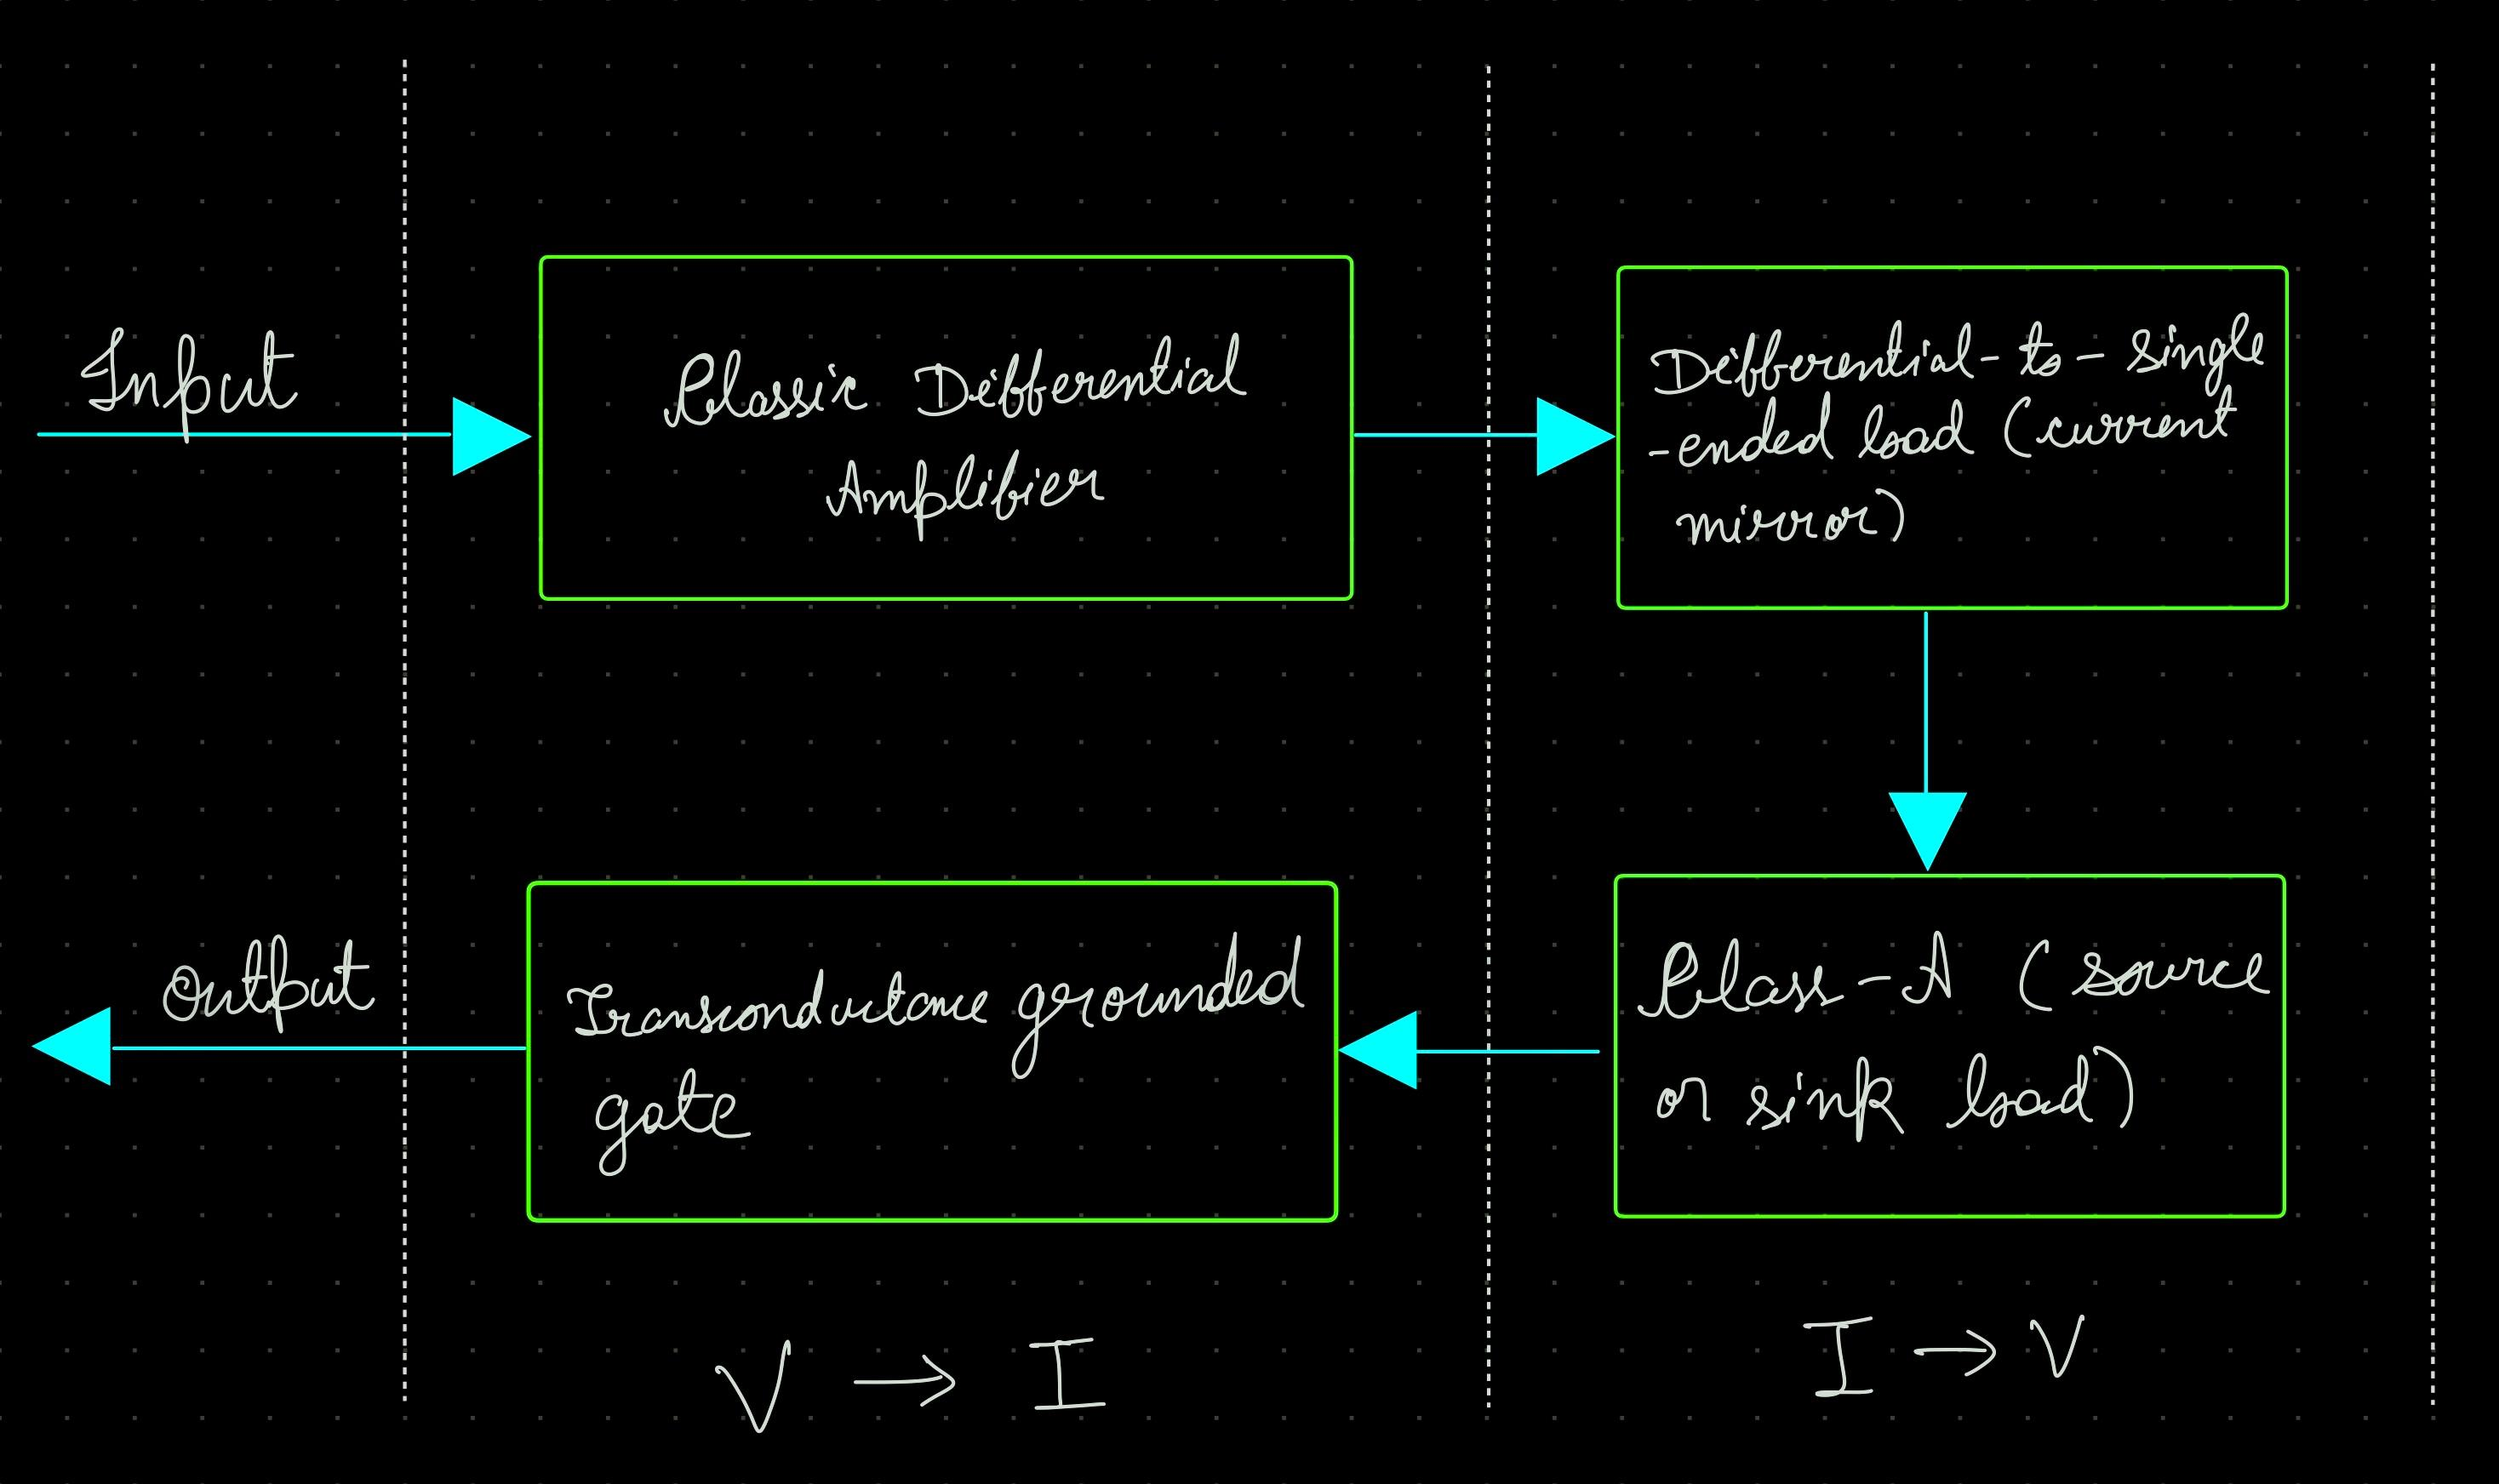
\includegraphics[keepaspectratio]{fig1a.jpeg}}

}

\subcaption{\label{fig-block}Block diagram of \(V \rightarrow I\) and
\(I \rightarrow V\) stages}

\end{minipage}%
%
\begin{minipage}[t]{0.50\linewidth}

\centering{

\pandocbounded{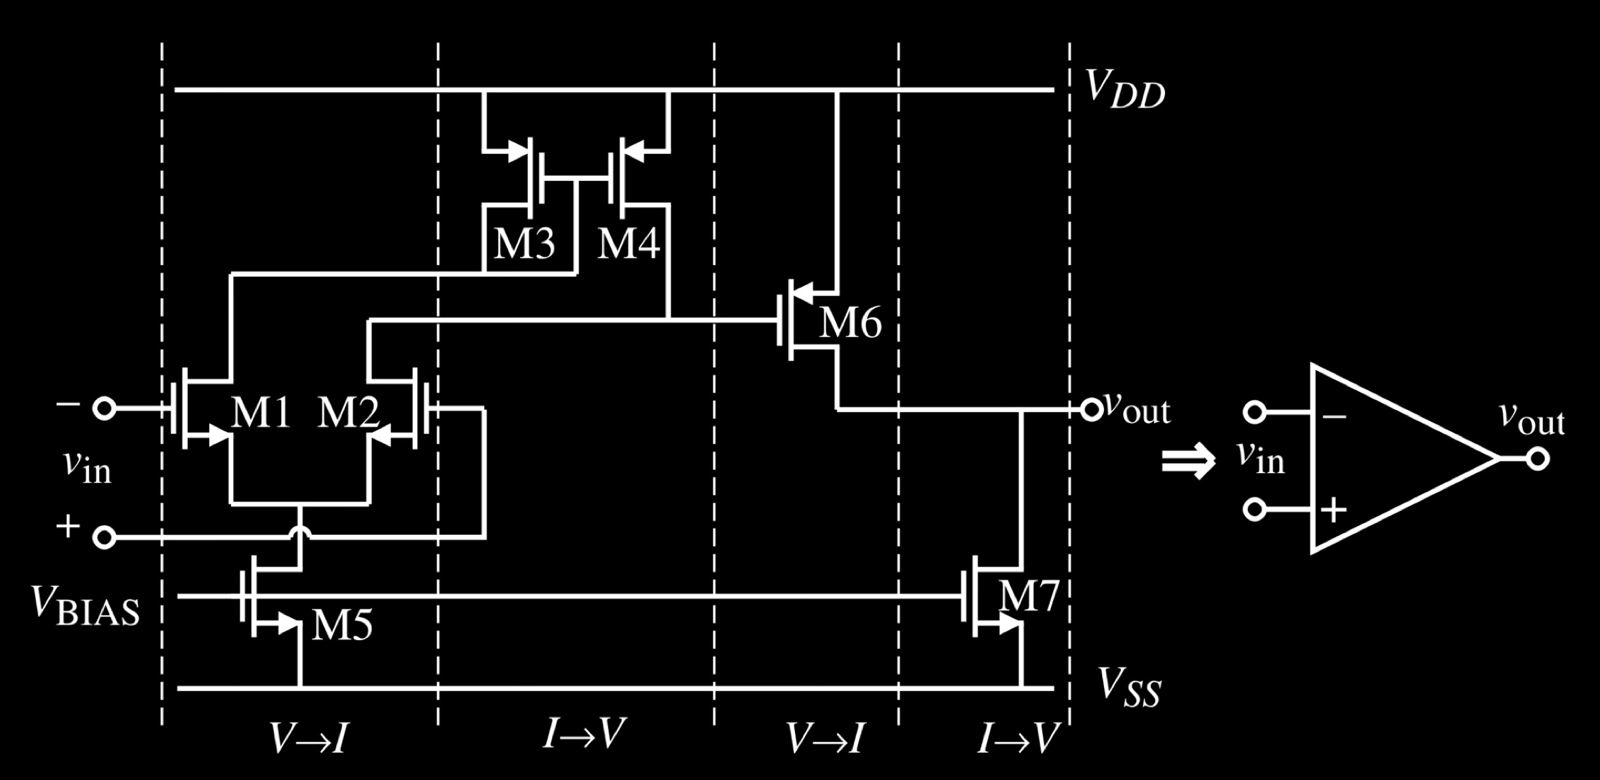
\includegraphics[keepaspectratio]{fig1b.png}}

}

\subcaption{\label{fig-transistor}Transistor level diagram. Adapted from
(Allen and Holberg 2011)}

\end{minipage}%

\caption{\label{fig-architecture}Architecture of the two-stage OTA.}

\end{figure}%

\section{Theoretical Design and
Calculations}\label{theoretical-design-and-calculations}

The design of op-amps can be divided into two distinct design related
activities that are for the most part independent of each other.

\begin{itemize}
\tightlist
\item
  The general schematic, which we have already decided above.
\item
  Calculating the DC currents, sizing up the transistors and designing
  the compensation network, based on the requirements.
\end{itemize}

The boundary conditions and requirements we will need to design our
op-amp:

\begin{itemize}
\item
  Boundary Conditions:

  \begin{enumerate}
  \def\labelenumi{\arabic{enumi}.}
  \tightlist
  \item
    Process Specification (\(V_{T}\), \(K'\), \(C_{ox}\), etc.)
  \item
    Supply Voltage and Range
  \end{enumerate}
\item
  Requirements:

  \begin{enumerate}
  \def\labelenumi{\arabic{enumi}.}
  \tightlist
  \item
    Gain
  \item
    Unity Gain Bandwidth
  \item
    Slew Rate
  \item
    Input Common-Mode range (\(ICMR\))
  \item
    Output-voltage swing
  \item
    Phase Margin
  \item
    Power Dissipation
  \end{enumerate}
\end{itemize}

In our first iteration, let us use the basic topology shown in Fig 2.

\begin{figure}

\centering{

\pandocbounded{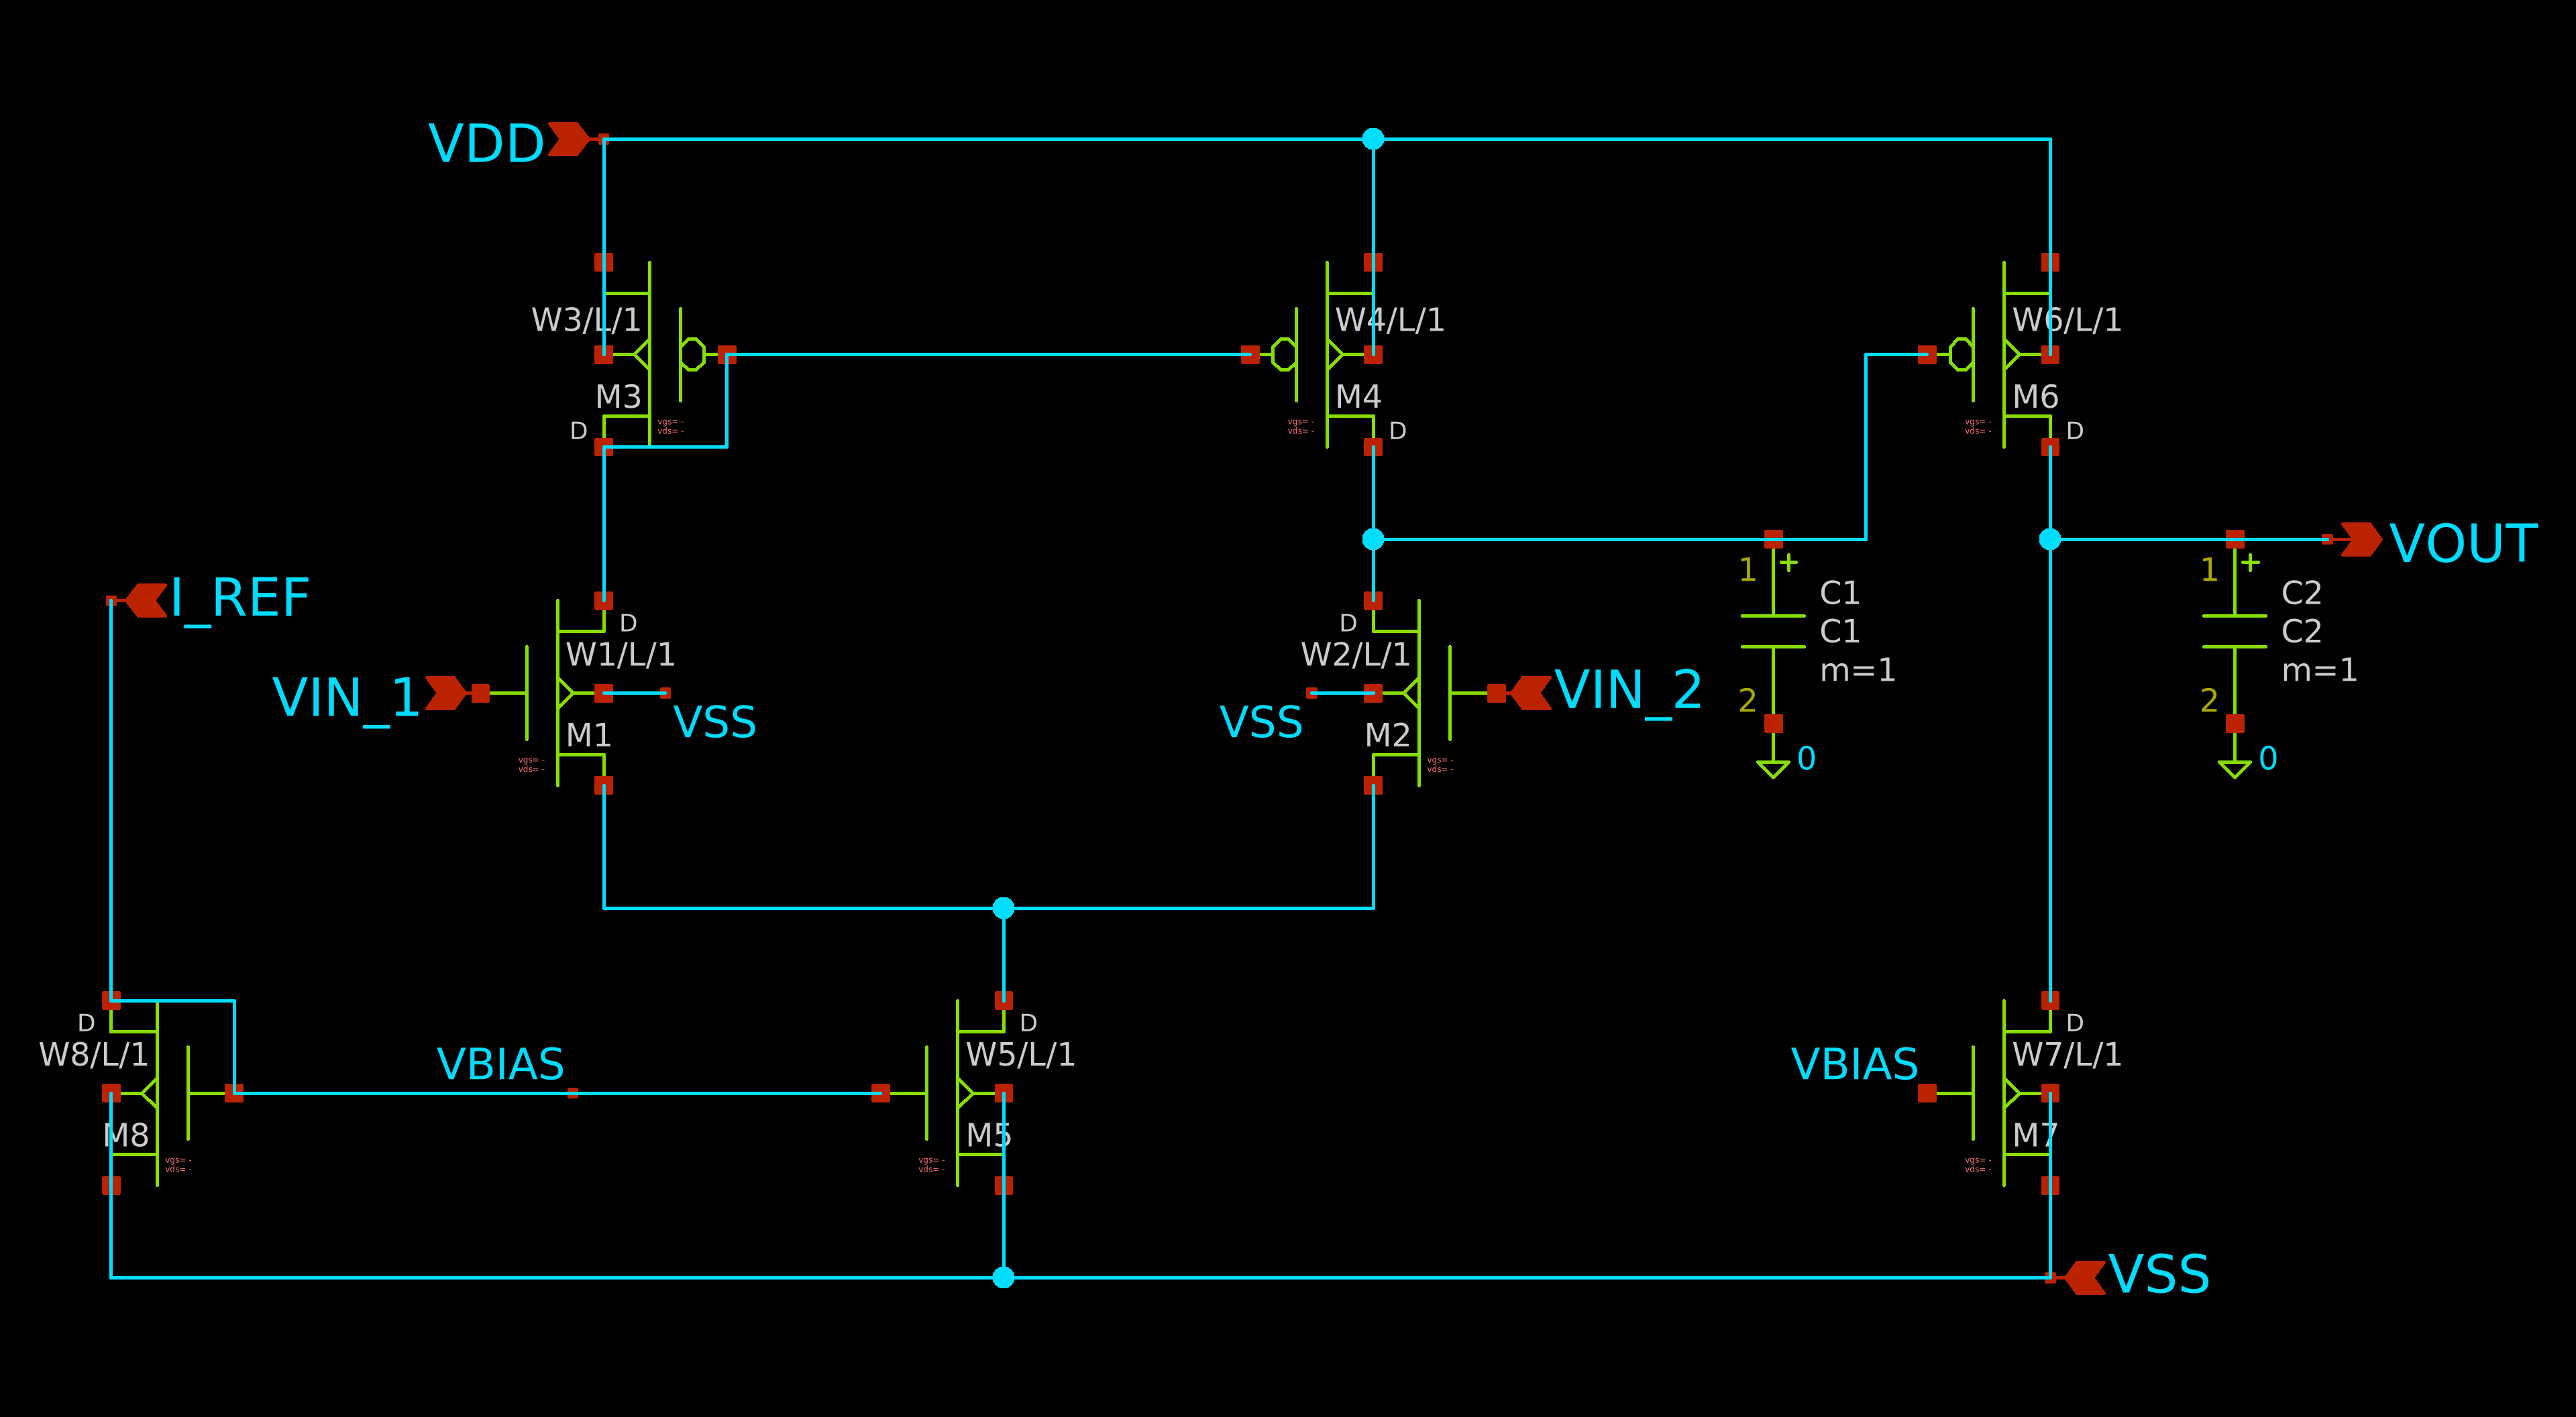
\includegraphics[keepaspectratio]{fig2.png}}

}

\caption{\label{fig-unique-name}Uncompensated Two-Stage CMOS OTA}

\end{figure}%

The small signal model for this circuit is shown in Fig 3.

\begin{figure}

\centering{

\pandocbounded{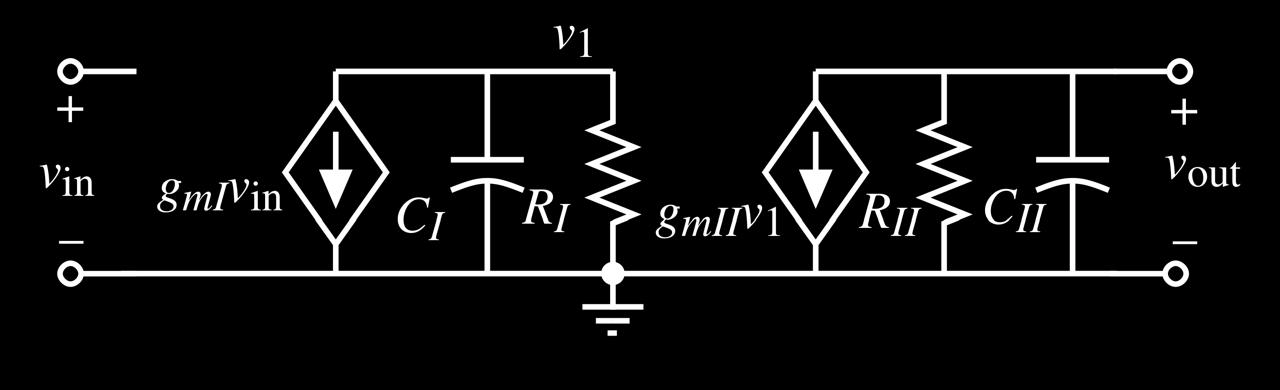
\includegraphics[keepaspectratio]{fig3.png}}

}

\caption{\label{fig-unique-name}Small Signal model of the uncompensated
OTA}

\end{figure}%

The locations of the two poles are given as:

\[
p'_{1} = (\frac{-1}{R_{I}.C_{I}})\] and, \[
p'_{2} = (\frac{-1}{R_{II}.C_{II}})\]

Where \(R_{I}\)/\(C_{I}\) and \(R_{II}\)/\(C_{II}\) are
resistance/capacitance to ground seen from the output of the first stage
and second stage respectively.

In a general case, these poles are far away from the origin and
relatively close together. Fig 4 illustrates the open-loop frequency
response of a negative-feedback loop op-amp in fig 2.

\begin{figure}[H]

{\centering \pandocbounded{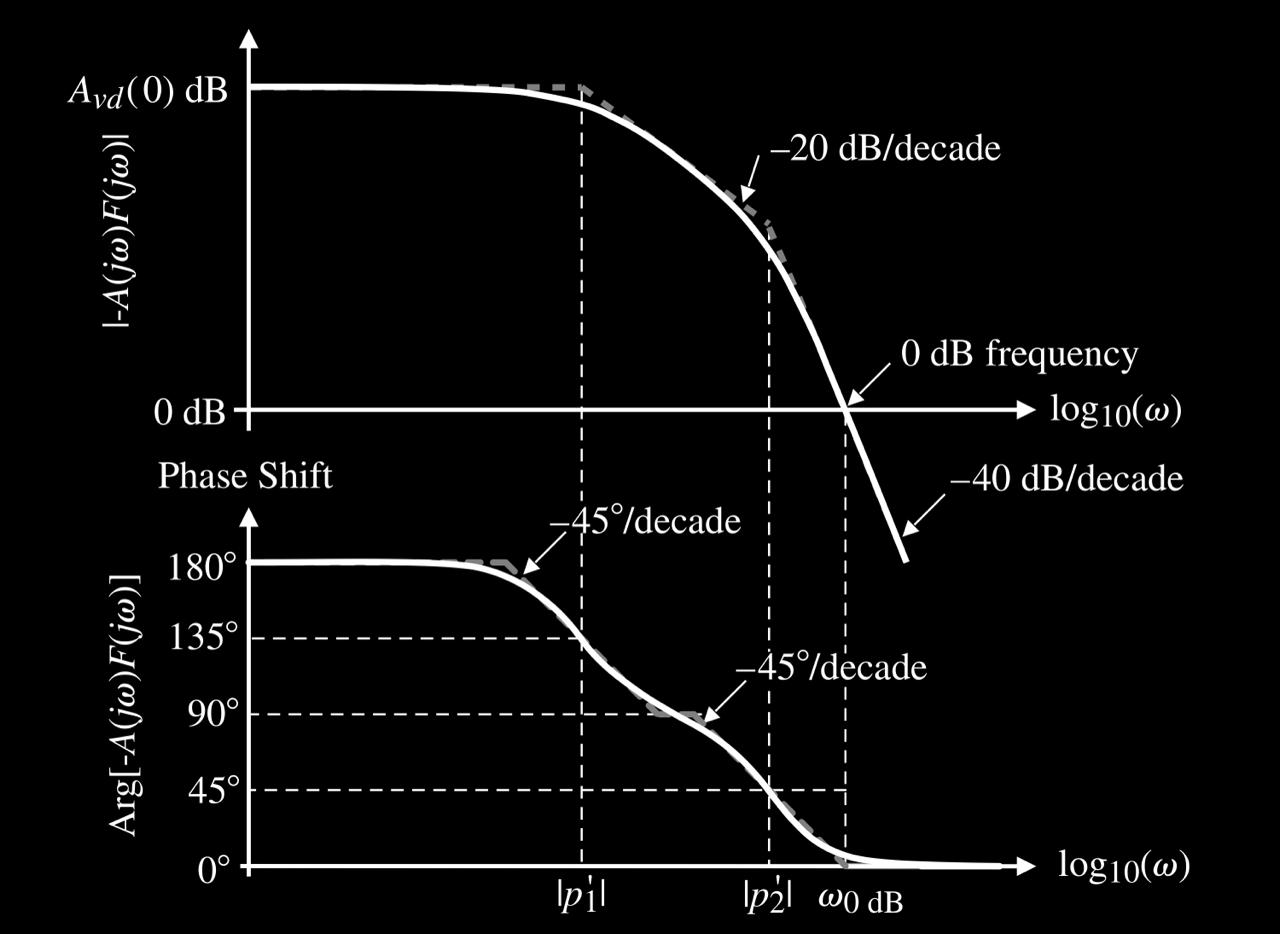
\includegraphics[keepaspectratio]{fig4.png}}

}

\caption{open-loop freq response of negative-feedback loop of
uncompensated op-amp}

\end{figure}%

As seen in Fig 4, the phase margin is significantly less than
\(45^{\circ}\), which will lead to instability. Thus, the op-amp needs
to be compensated before using it in a closed loop configuration.

\subsection{Miller Compensation}\label{miller-compensation}

Adding the compensation capacitor \(C_{c}\), the resulting circuit is
shown in Fig 5:

\begin{figure}[H]

{\centering \pandocbounded{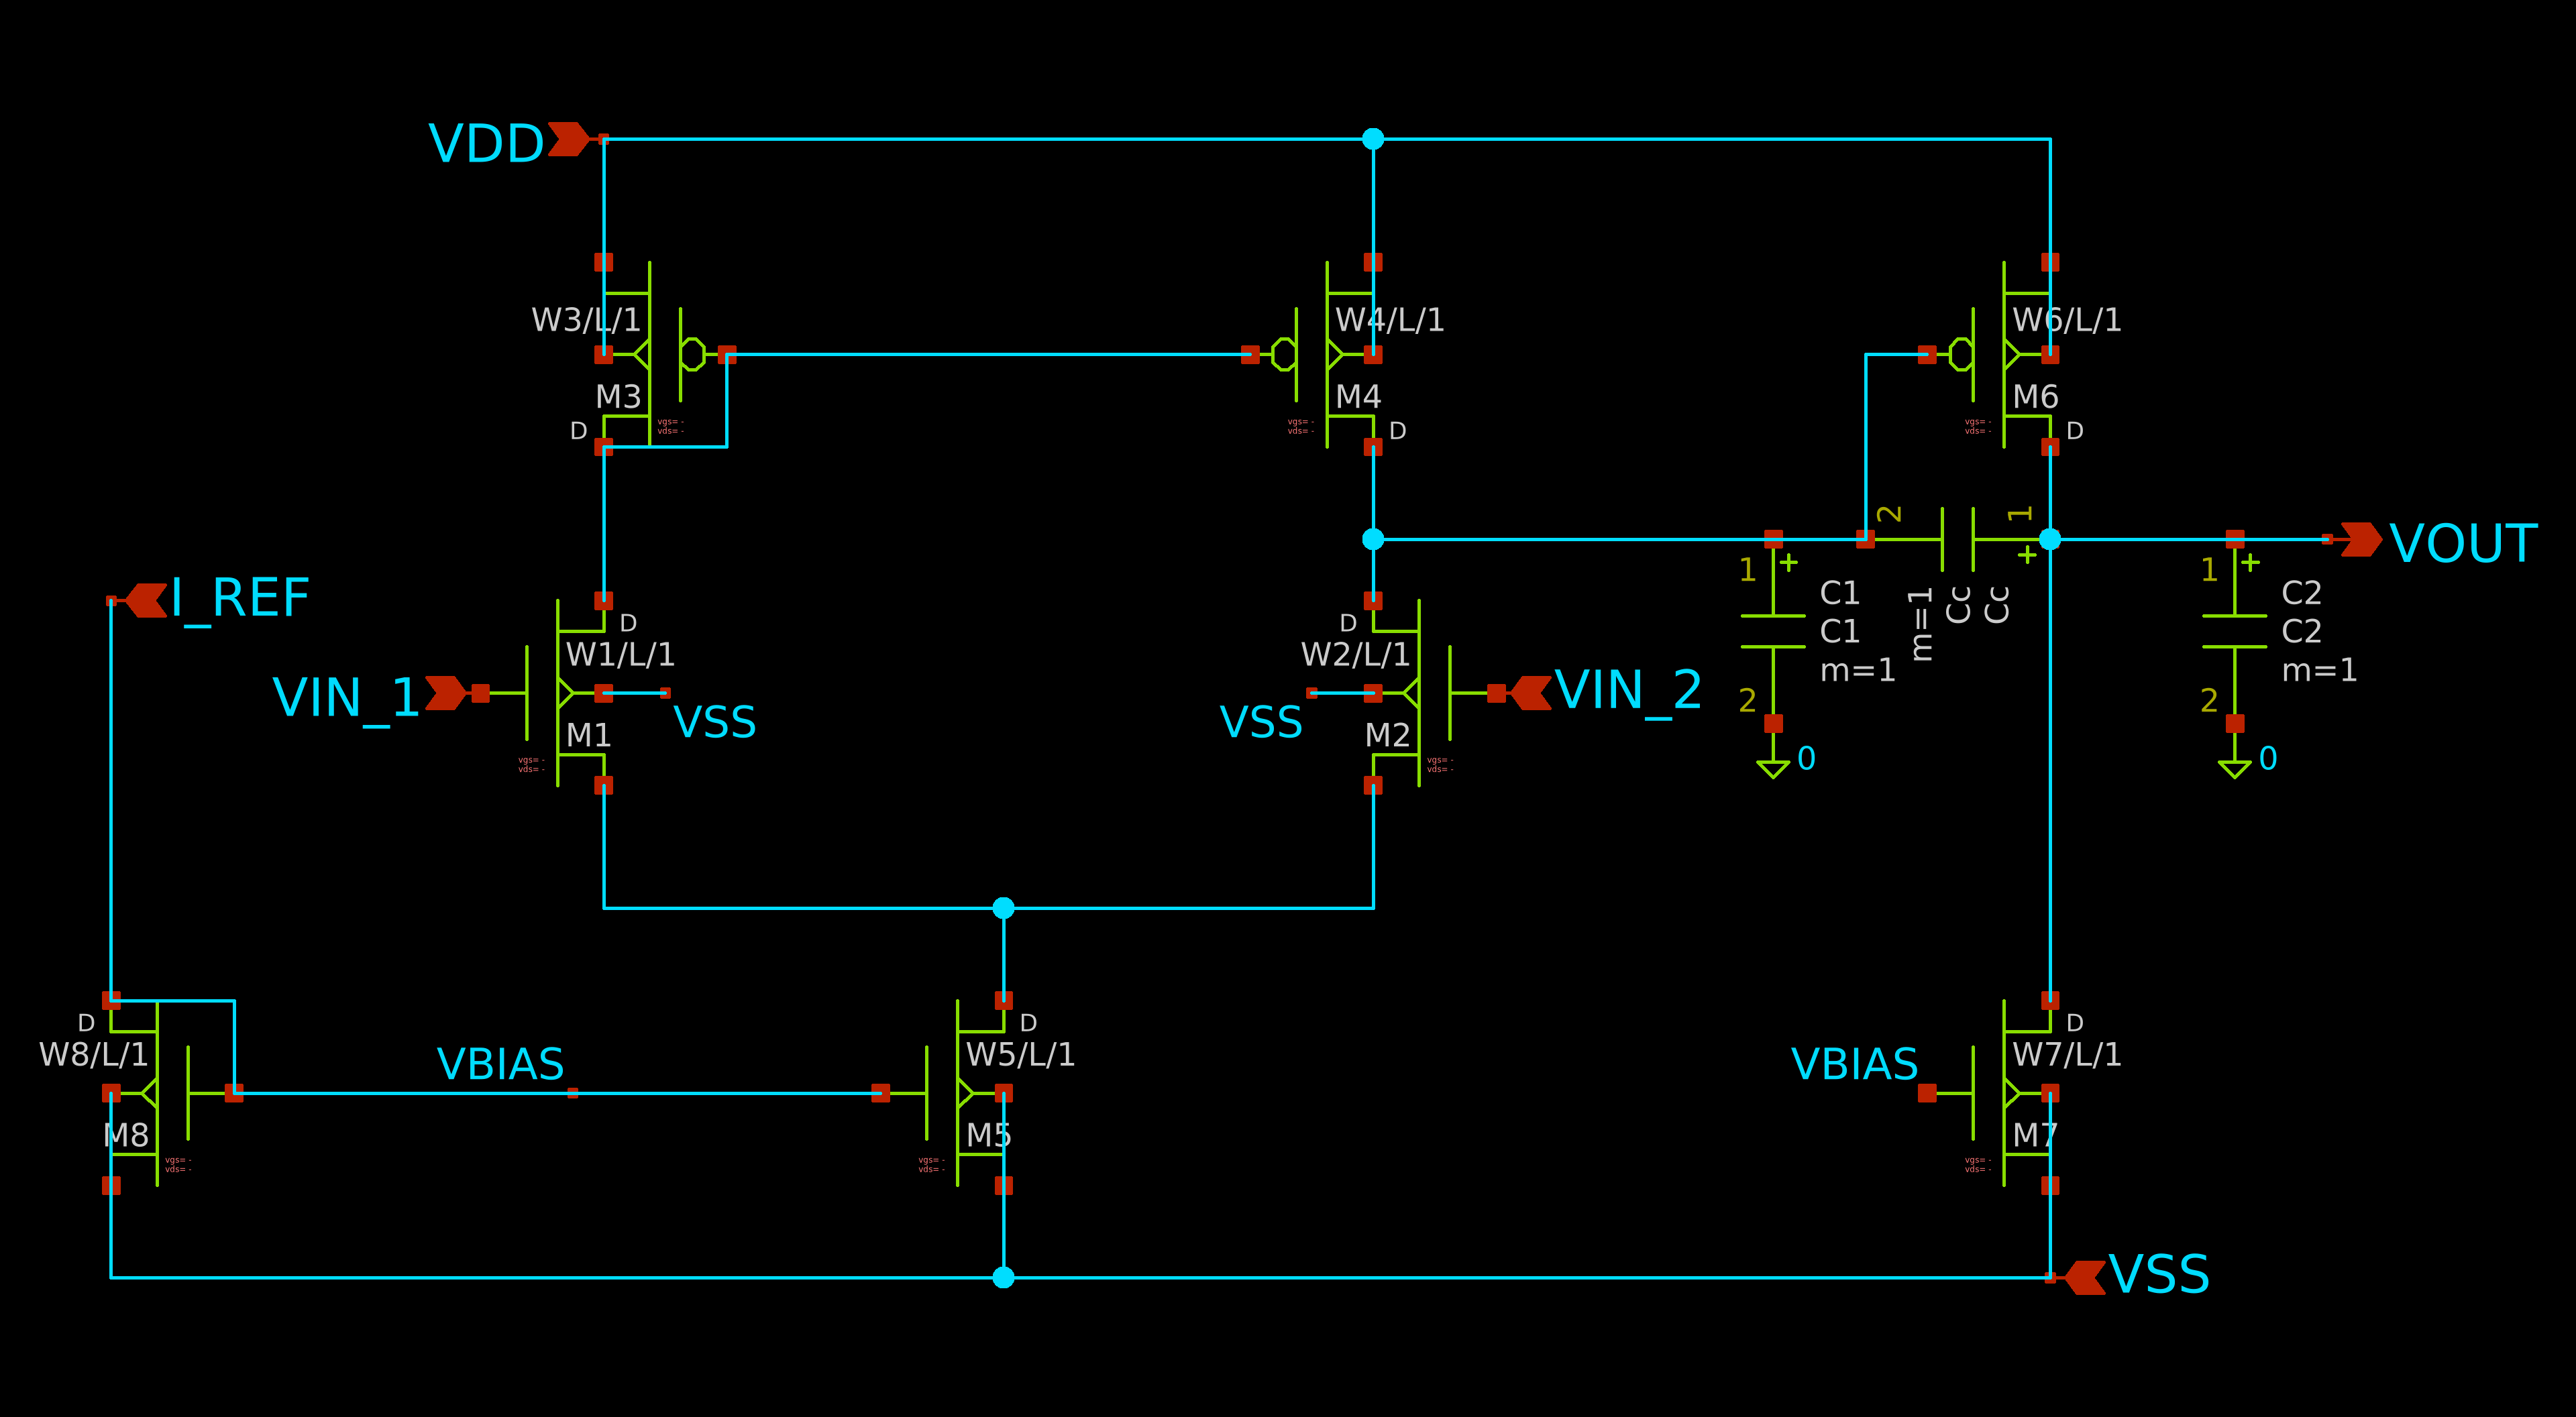
\includegraphics[keepaspectratio]{fig5.png}}

}

\caption{Compensated two-stage op-amp}

\end{figure}%

The resulting small-signal model is shown in Fig 6:

\begin{figure}[H]

{\centering \pandocbounded{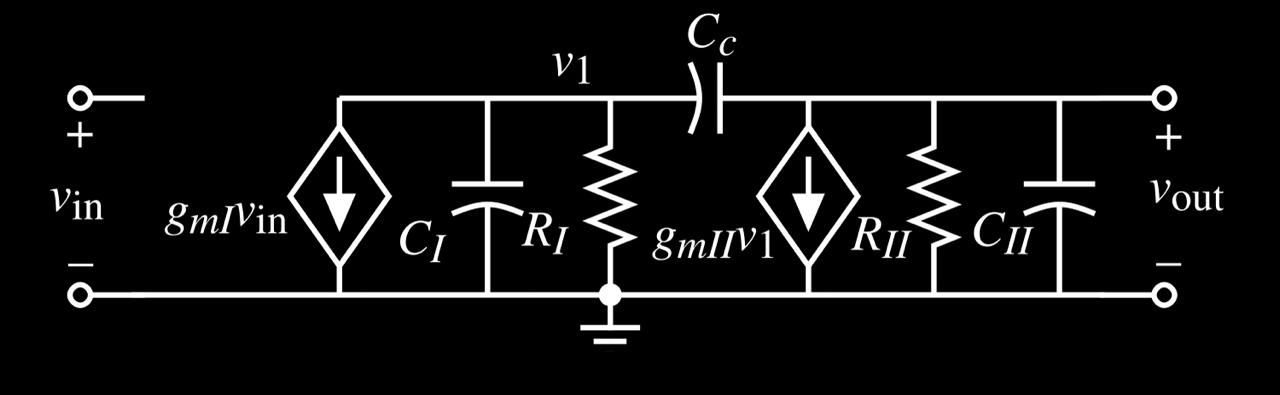
\includegraphics[keepaspectratio]{fig6.png}}

}

\caption{small-signal model of compensated two-stage op-amp}

\end{figure}%

Using Miller's Approximation and finding poles by inspection, we have

\(`\ p_{1} \approx (\frac{-1}{R_{I}.[C_{I} + C_{c}(1 + g_{mII}.R_{II})]})`\)

\(`\ p_{2} \approx (\frac{-g_{mII}}{C_{II} + C_{c}}) \approx (\frac{-g_{mII}}{C_{II}}) ;\space if \space C_{II} > C_{c}`\)

A zero also occurs on the positive real axis, which can be found from
the small signal model relatively easily by setting \(A_{v} = 0\)

\(`\ z_{1} = (\frac{g_{mII}}{C_{c}}) `\)

The addition of miller capacitance moves the dominant pole \((p_{1})\)
to the left and shifts the non dominant pole \((p_{2})\) to the right.

If we use our assumption of \(C_{II} > C_{c}\), then the zero is further
to the right of \((p_{2})\)

Fig 7 shows results of compensation compared to the uncompensated state.

\begin{figure}[H]

{\centering \pandocbounded{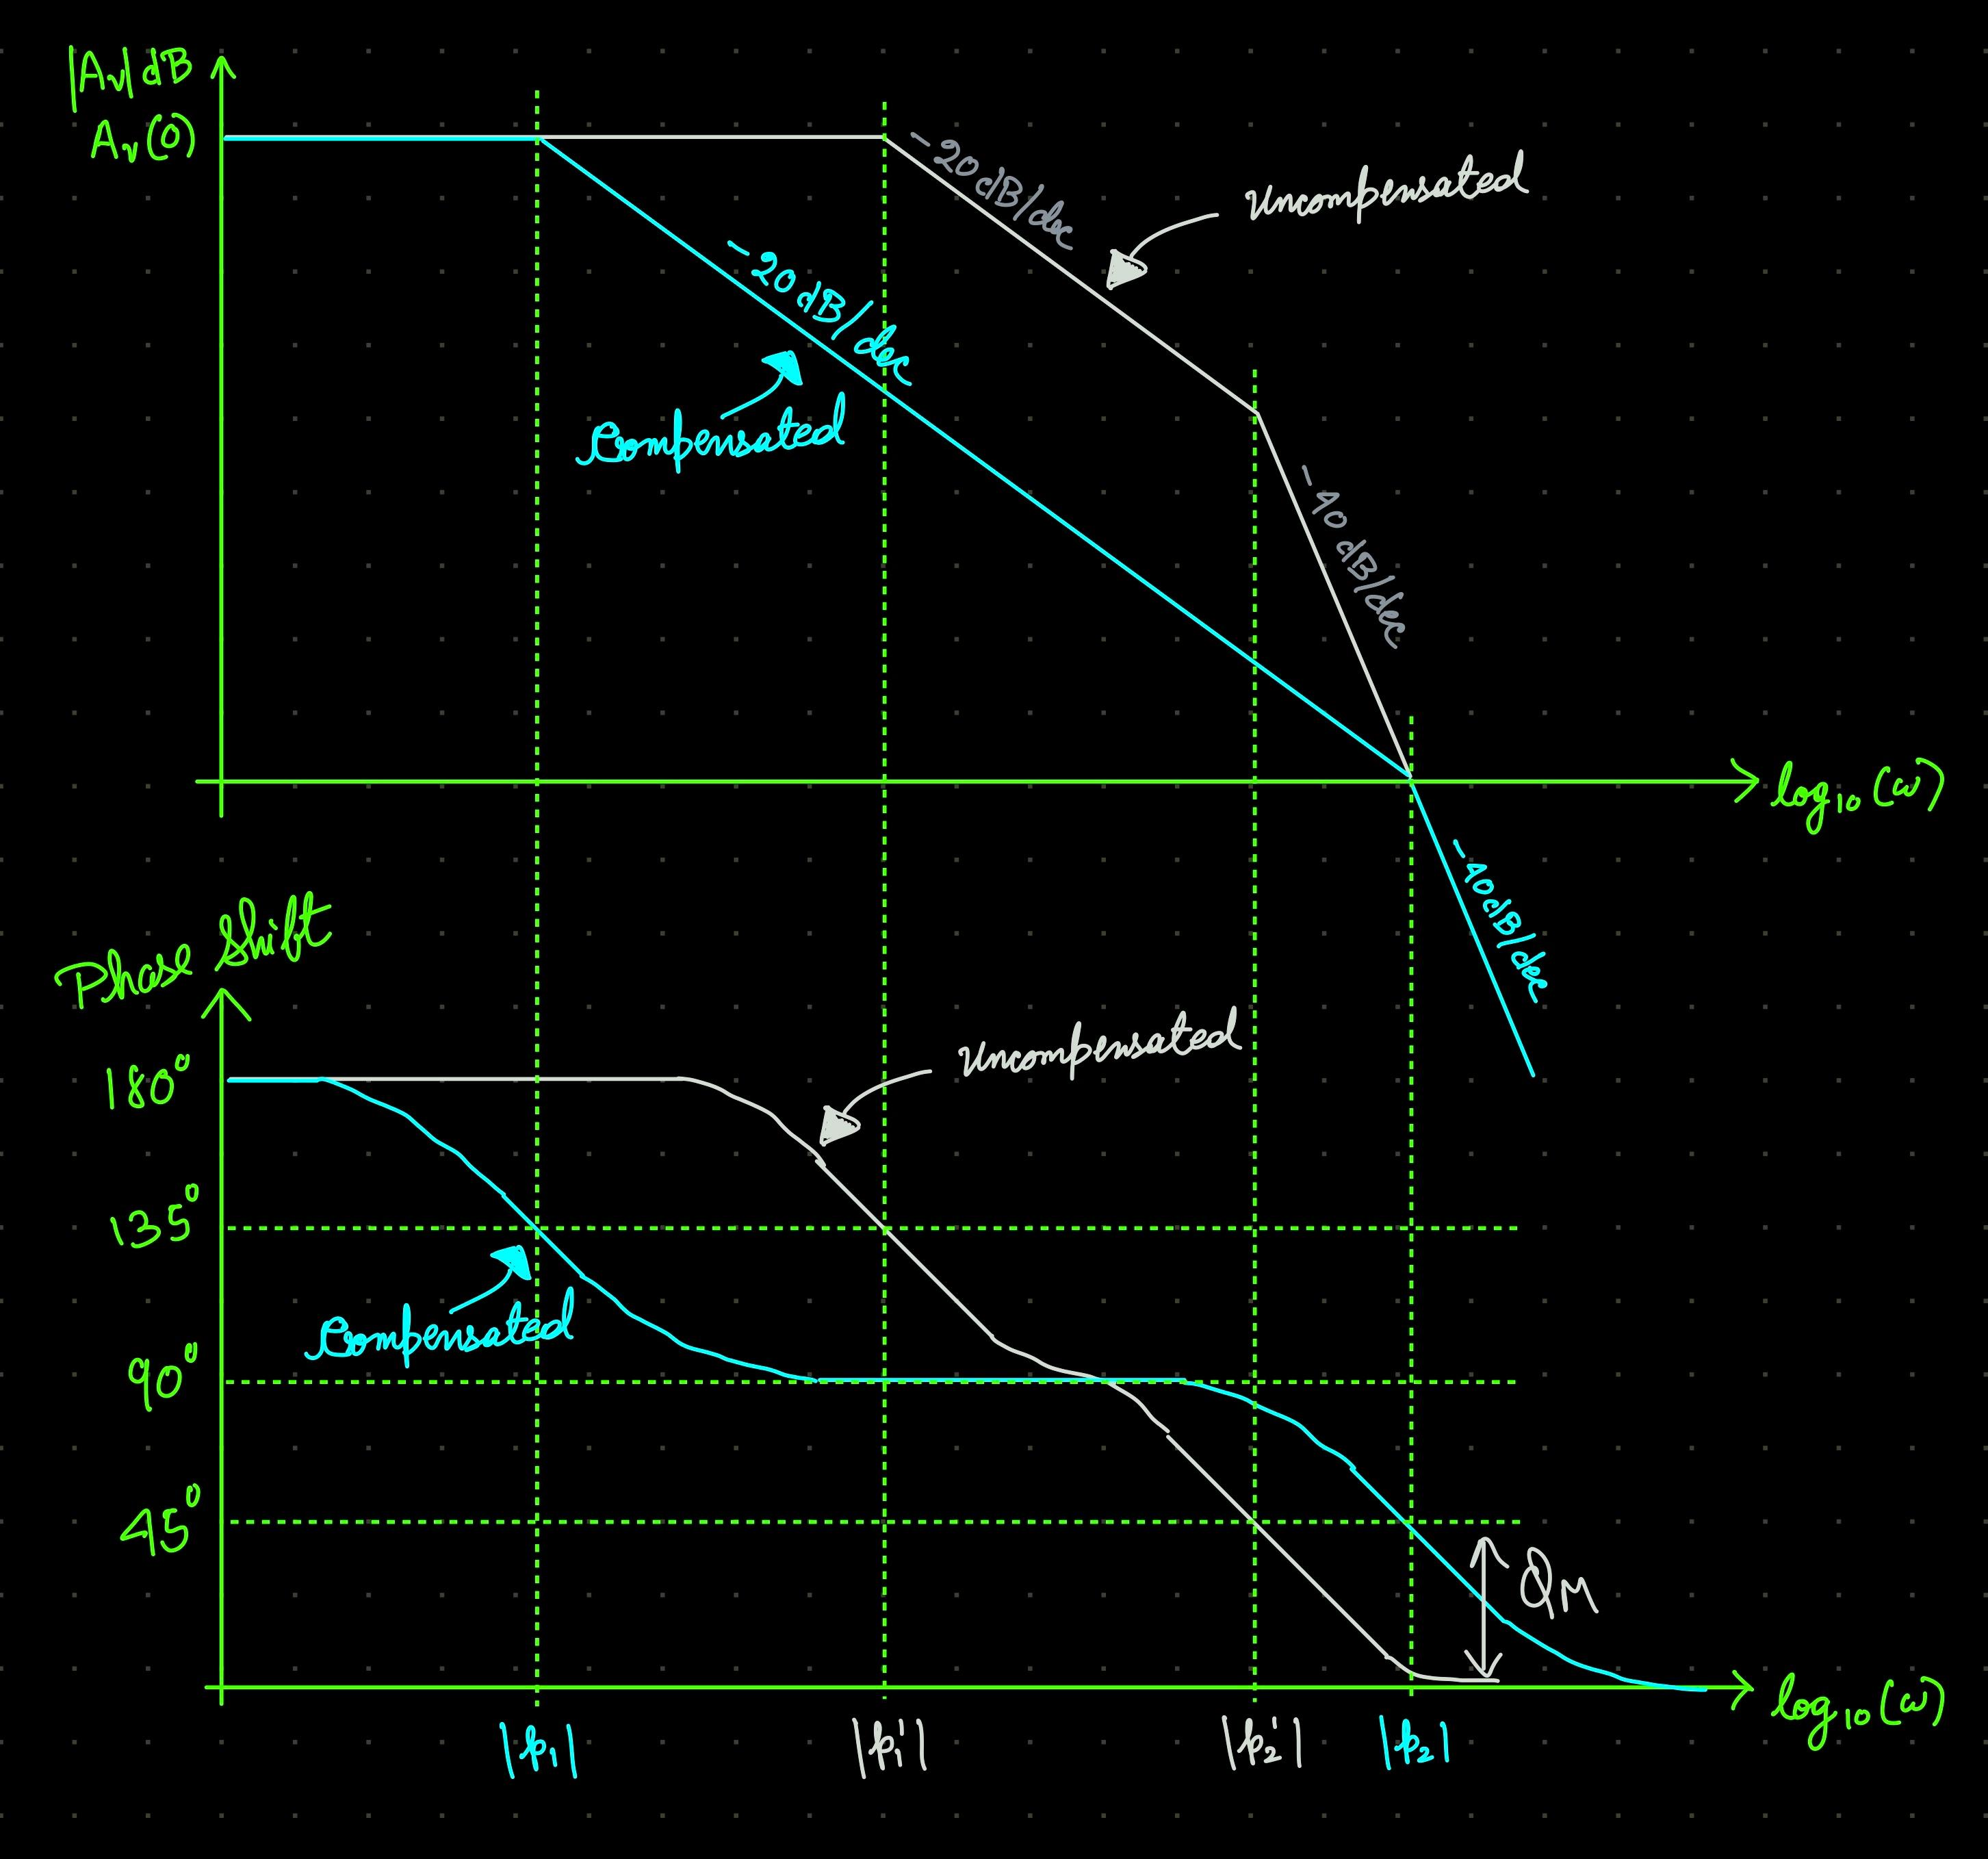
\includegraphics[keepaspectratio]{fig7.jpeg}}

}

\caption{compensated op-amp}

\end{figure}%

The \textbf{unity gain bandwidth} is defined as the angular frequency
(or frequency) when the gain crosses the \(0dB\) mark. It is given as:

\(`(\omega_{GBW}) \approx (\frac{g_{mI}}{C_{c}})`\)

If we define \(z_{1} > 10.{\omega_{GBW}}\), then, to achieve
\(\phi_{M} > 60^{\circ}\), we need the following condition:

\begin{itemize}
\tightlist
\item
  \(p_{2} > 2.2.{\omega_{GBW}}\)\\
  OR
\item
  \(C_{c} > 0.22.C_{2}\)
\end{itemize}

\subsection{Component Sizing}\label{component-sizing}

Before beginning, let us summarise the important relationships:

\begin{enumerate}
\def\labelenumi{\arabic{enumi}.}
\item
  First Stage Gain:
  \[ A_{v1} = \frac{-g_{m1}}{g_{ds2} + g_{ds4}} = \frac{-2.g_{m1}}{I_{5}.(\lambda_{2} + \lambda_{4})} \]
\item
  Second Stage Gain:
  \[ A_{v2} = \frac{-g_{m2}}{g_{ds6} + g_{ds7}} = \frac{-2.g_{m2}}{I_{6}.(\lambda_{6} + \lambda_{7})} \]
\item
  Unity Gain Bandwidth:

  \[\omega_{GBW} \approx \frac{g_{m2}}{C_{c}}\]
\item
  Slew Rate: \$ SR = \frac{I_{5}}{C_{c}} \$
\item
  \(ICMR+ (V_{in}(max)) = V_{DD} - \sqrt{\frac{I_{5}}{K'(\frac{W}{L})_{3}}} - |V_{T03}|(max) + V_{T1}(min)\)
\item
  \(ICMR- (V_{in}(min)) = V_{SS} + \sqrt{\frac{I_{5}}{K'(\frac{W}{L})_{1}}} + V_{T1}(max) + V_{DS5}(sat)\)
\item
  Saturation Voltage: \$ V\_\{DS5\}(sat) =
  \sqrt{\frac{2.I_{DS}}{K'(\frac{W}{L})}} \$
\end{enumerate}

Going onto the design procedure, a first cut sequence we can follow is:

\begin{itemize}
\item
  The design procedure begins by choosing a device length to be used by
  the circuit. This length determines the channel length modulation
  parameter \((\lambda)\), which is necessary to calculate amplifier
  gain.
\item
  Keeping our definition of \(z_{1} > 10.{\omega_{GBW}}\), minimum value
  of \(C_{c}\) can be defined as: \(C_{c} > 0.22.C_{2}\)
\item
  Next, minimum value of tail current \((I_{5})\) can be determined by
  \$ I\_\{5\} = SR.C\_\{c\} \$
\item
  \$ (\frac{W}{L})\emph{\{3\} = (}\frac{W}{L})\{4\} =
  \frac{I_{5}}{(K'_{3}).(ICMR+)^{2}} \$
\item
  \$ g\_\{m1\} = g\_\{m2\} = \{\omega*\{GBW\}\}.C*\{c\} \$
\item
  \$ V\_\{DS5\} = (ICMR-) - V\_\{SS\} -
  \sqrt{\frac{I_{5}}{K'(\frac{W}{L})_{1}}} - V\_\{T1\}(max) \$
\item
  \$ (\frac{W}{L})\_\{5\} = \frac{2.I_{5}}{K'_{5}.(V_{DS5})^{2}} \$
\item
  Again, following \(z_{1} > 10.{\omega_{GBW}}\), we have: \$ g\_\{m6\}
  = 2.2(g\_\{m2\})(\frac{C_{L}}{C_c}) \$
\item
  \$ (\frac{W}{L})\emph{\{6\} =
  (}\frac{W}{L})\{4\}.(\frac{g_{m6}}{g_{m4}}) \$
\item
  \$ I\_\{6\} = \frac{g_{m6}^{2}}{2.K'_{6}.(\frac{W}{L})_{6}} \$
\item
  \$ (\frac{W}{L})\emph{\{7\} =
  (}\frac{W}{L})\{5\}.(\frac{I_{6}}{I_{5}})\$
\item
  \$ P\_\{dis\} = (I\_\{5\} + I\_\{6\} + I\_\{8\}).(V\_\{DD\} +
  \textbar V\_\{SS\}\textbar) \$
\item
  Now, the gain must be checked against the specifications, if it is too
  low, \(I_{5}\) and \(I_{6}\) may be decreased or the ratios
  \((\frac{W}{L})_{2}\) and \((\frac{W}{L})_{6}\) may be increased. All
  the previous calculations need to be performed again to ensure all
  conditions are satisfied.
\end{itemize}

\subsection{Biasing Network}\label{biasing-network}

\begin{itemize}
\item
  A current mirror approach with a stable reference current (say, using
  \(\beta-Multiplier\)) is used to bias the current sink \(M_{7}\) and
  tail current source \(M_{5}\)

  \begin{itemize}
  \tightlist
  \item
    Since \(M_{8}\) acts as our reference current mirror, we can have \$
    (\frac{W}{L})\emph{\{8\} = (}\frac{W}{L})\{5\} \$ to set \$
    I\_\{tail\}=I\_\{ref\} \$, and the relation of \$
    (\frac{W}{L})\emph{\{5\} \$ with \$ (}\frac{W}{L})\{7\} \$ is known
    from above calculations.
  \end{itemize}
\item
  The Bias Point of the differential input is found as:

  \begin{itemize}
  \tightlist
  \item
    \$ g\_m = \frac{2I_{D}}{V_{ov}} \$
  \item
    \$ \textbar A\_\{v1\}\textbar{} = \frac{g_{m1}}{g_{ds2} + g_{ds4}} =
    \frac{2}{V_{ov}.(\lambda_{2}+\lambda_{4})} \$
  \item
    \$ V\_\{ov\} = \frac{2}{|A_{v1}|.(\lambda_{2}+\lambda_{4})} \$
  \end{itemize}
\end{itemize}

\subsection{Requirements and
Specifications}\label{requirements-and-specifications}

The specifications we will use are as follows:

\begin{itemize}
\tightlist
\item
  \$ A\_\{v\} \textgreater{} 5000 V/V \$
\item
  \$ \{\omega\_\{GBW\}\} = 5MHz \$
\item
  \(\phi_{M} > 60^{\circ}\)
\item
  \(ICMR- = -1V\)
\item
  \(ICMR+ = 2V\)
\item
  \(SR > 10V/us\)
\item
  \(V_{out} \pm2V\)
\item
  \(V_{DD} = 2.5V\)
\item
  \(V_{SS} = -2.5V\)
\item
  \(C_{L} = 10pF\)
\item
  \(P_{dis} < 2mW\)
\item
  \(L = 1um\)
\end{itemize}

The important process parameters from the model used are:

\begin{itemize}
\tightlist
\item
  \$ K'\_\{n\} = 120uA/V\^{}\{2\} \$
\item
  \$ V\_\{TN\} = 0.8V \$
\item
  \$ K'\_\{p\} = 40uA/V\^{}\{2\} \$
\item
  \$ V\_\{TP\} = -0.9V \$
\end{itemize}

\subsection{Initial Sizing}\label{initial-sizing}

Following the design procedure and substituting the values from
requirements and process parameters, the initial calculated values are:

\begin{itemize}
\tightlist
\item
  \$ C\_\{c\} = 3pF \$
\item
  \$ I\_\{5\} = 30uA \$
\item
  \$ (\frac{W}{L})\emph{\{3\} = (}\frac{W}{L})\{4\} \approx 10 \$
\item
  \$ g\_\{m1\} = g\_\{m2\} = 94.2uS \$
\item
  \$ g\_\{m3\} = g\_\{m4\} = 109uS \$
\item
  \$ (\frac{W}{L})\emph{\{1\} = (}\frac{W}{L})\{2\} \approx 3 \$
\item
  \$ V\_\{DS5\}(sat) = 0.411 \$
\item
  \$ (\frac{W}{L})\_\{5\} \approx 3 \$
\item
  \$ g\_\{m6\} = 942uS \$
\item
  \$ (\frac{W}{L})\_\{6\} \approx 86.6 \$
\item
  \$ I\_\{6\} = 130uA \$
\item
  \$ (\frac{W}{L})\_\{7\} \approx 13 \$
\item
  \$ V\_\{CM\} = 1.118V \$
\item
  \$ A\_\{v\} \approx 5600 \$
\item
  \$ P\_\{dis\} = 0.95mW \$
\end{itemize}

These initial values were entered into xschem and simulated. The
following sections document the schematic implementation, challenges
encountered in measuring the open-loop gain and the iterative
refinements made to meet all specifications.

\subsection{Pre-Simulation Results}\label{pre-simulation-results}

Based on the napkin math above, the following performace is expected:

{\def\LTcaptype{none} % do not increment counter
\begin{longtable}[]{@{}lll@{}}
\toprule\noalign{}
Parameter & Predicted Value & Specification \\
\midrule\noalign{}
\endhead
\bottomrule\noalign{}
\endlastfoot
DC Gain & \(\approx74.9 dB (5600 V/V)\) & \(> 73.98 dB (5000 V/V)\) \\
GBW & \(5 MHz\) & \(5 MHz\) \\
Phase Margin & \(> 60^{\circ}\) & \(> 60^{\circ}\) \\
Slew Rate & \(10 V/μs\) & \textgreater{} \(10 V/μs\) \\
Power & \(0.95mW\) & \textless{} \(2mW\) \\
\end{longtable}
}

\subsection{Schematic Implementation}\label{schematic-implementation}

The circuit was implemented in xschem with ngspice using Level 3 SPICE
model with 1um channel length. The complete schematic is shown in Fig 8.

\emph{Source for model: https://cmosedu.com/cmos1/cmosedu\_models.txt}

\begin{figure}[H]

{\centering \pandocbounded{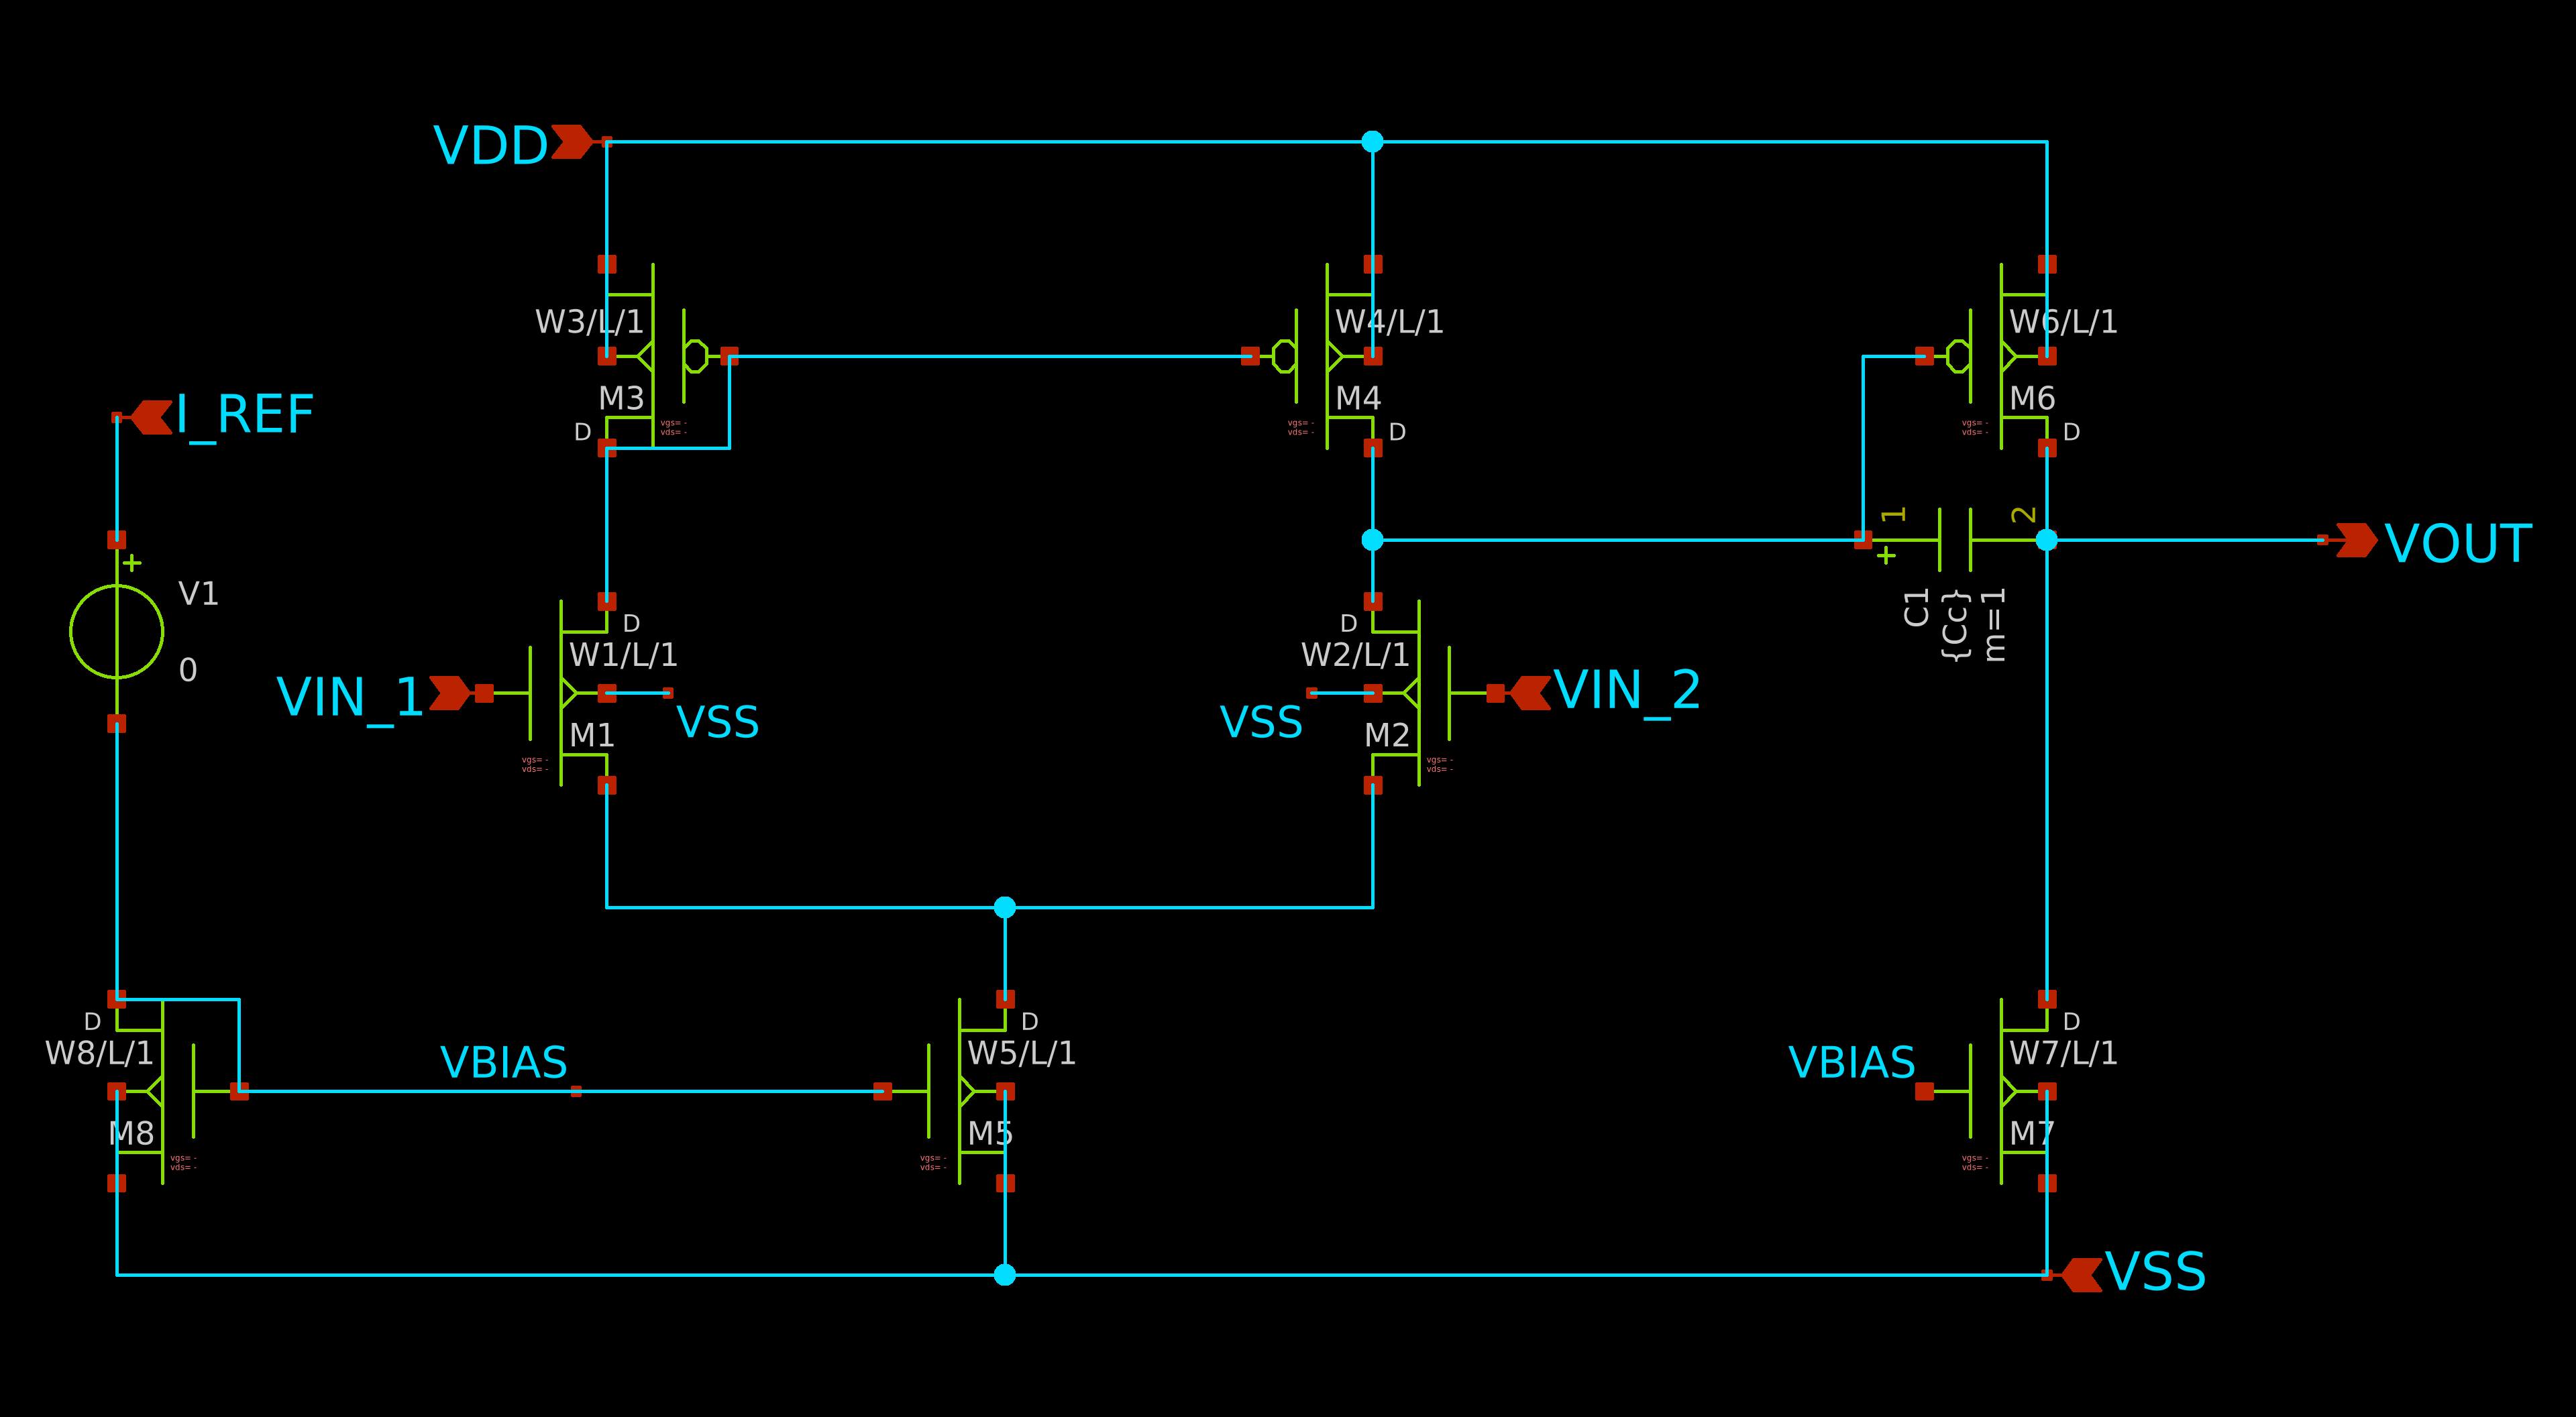
\includegraphics[keepaspectratio]{opamp_scheme.png}}

}

\caption{Full OTA Schematic}

\end{figure}%

The final transistor sizing after all iterations is summarised in the
table below:

{\def\LTcaptype{none} % do not increment counter
\begin{longtable}[]{@{}lll@{}}
\toprule\noalign{}
Transistor & Type & W/L \\
\midrule\noalign{}
\endhead
\bottomrule\noalign{}
\endlastfoot
M1, M2 & NMOS & 3.5 \\
M3, M4 & PMOS & 10 \\
M5 & NMOS & 3 \\
M6 & PMOS & 86.6 \\
M7 & NMOS & 13 \\
M8 & NMOS & 3 \\
\end{longtable}
}

Component values: \(C_c = 2.5pF\), \(C_L = 10pF\)

\begin{center}\rule{0.5\linewidth}{0.5pt}\end{center}

\section{Simulation Results}\label{simulation-results}

\subsection{DC Operating Point}\label{dc-operating-point}

All transistors were verified to be in saturation before AC analysis.
The testbench is shown in Fig 9.

\begin{figure}[H]

{\centering \pandocbounded{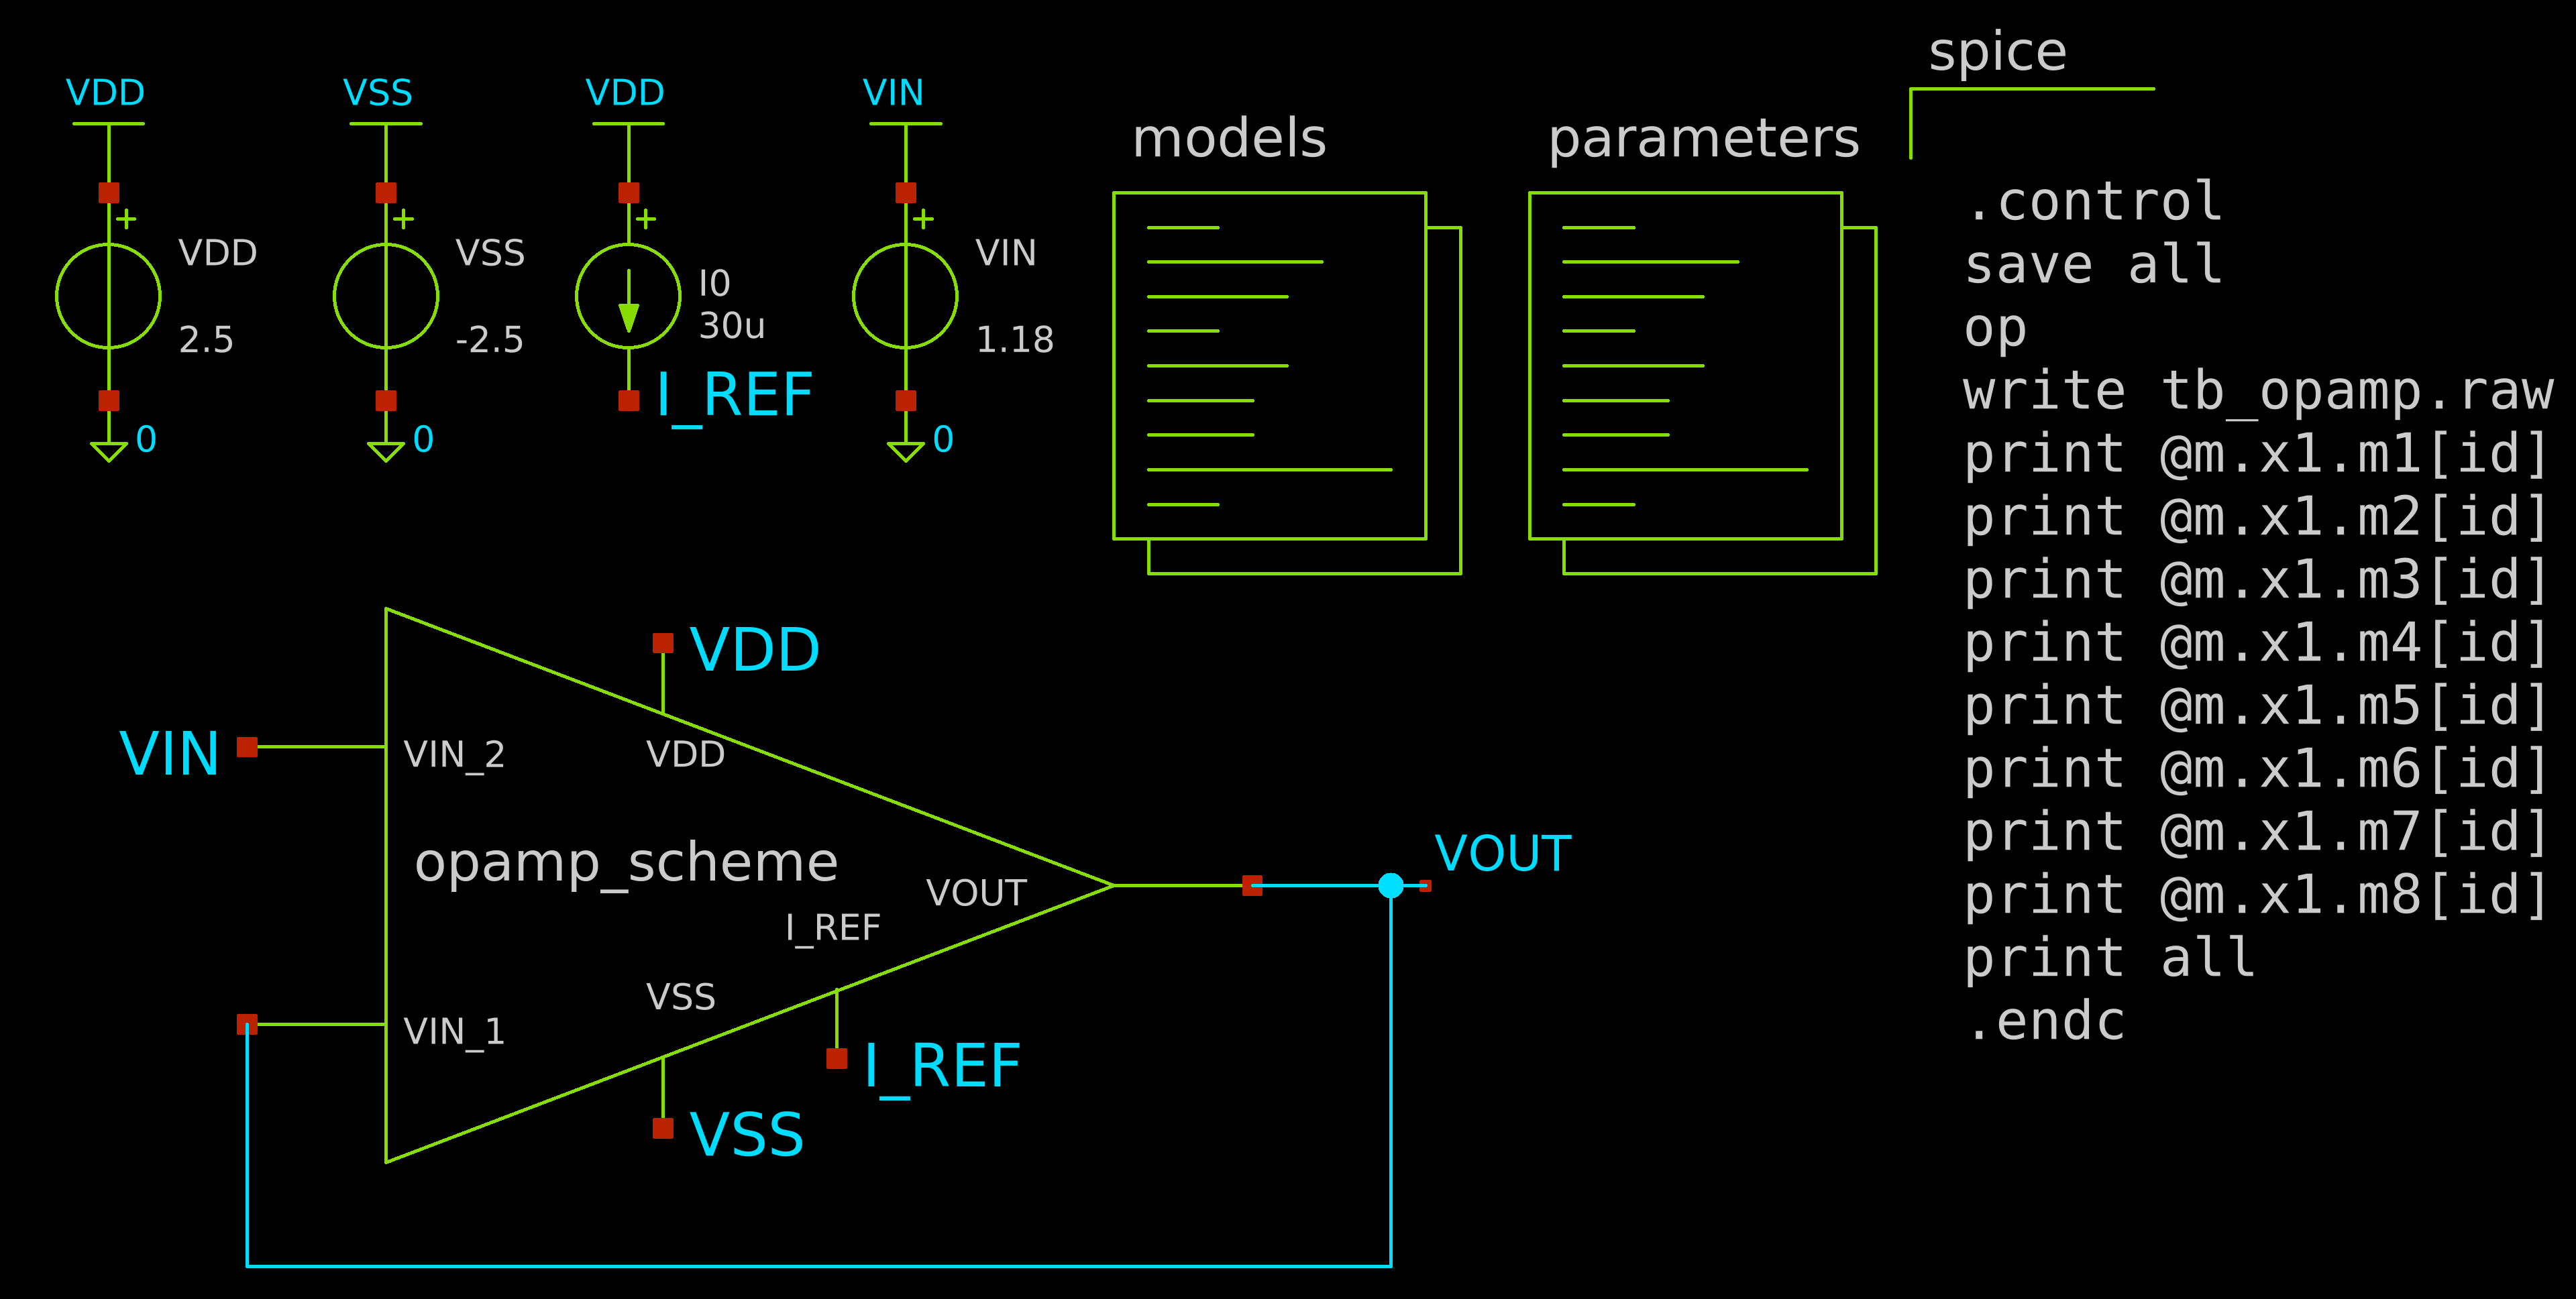
\includegraphics[keepaspectratio]{tb_opamp.png}}

}

\caption{alt text}

\end{figure}%

{\def\LTcaptype{none} % do not increment counter
\begin{longtable}[]{@{}llll@{}}
\toprule\noalign{}
Transistor & \(\|V_{ov}\|\) & \(\|V_{DS}\|\) & Region \\
\midrule\noalign{}
\endhead
\bottomrule\noalign{}
\endlastfoot
M1 & 0.745 & 1.748 & Saturation \\
M2 & 0.745 & 1.706 & Saturation \\
M3 & 0.216 & 1.116 & Saturation \\
M4 & 0.216 & 1.159 & Saturation \\
M5 & 0.463 & 2.134 & Saturation \\
M6 & 0.259 & 1.320 & Saturation \\
M7 & 0.463 & 3.679 & Saturation \\
M8 & 0.463 & 1.263 & Saturation \\
\end{longtable}
}

\subsection{Open-Loop Gain (AC
Analysis)}\label{open-loop-gain-ac-analysis}

Simulation of measurement of open-loop gain of op-amp is a difficult
step to perform. The reason is the high differential gain in op-amps.

In our case, with a gain of \textasciitilde5000V/V, any offset voltage
present is amplified by \(5000.V_{OS}\) at the output. So, for any
\(V_{OS} < 0.5mV\), the output is driven to the maximum output swing
possible, making it difficult to measure the open loop gain. This is
shown in Fig 10.

\begin{figure}[H]

{\centering \pandocbounded{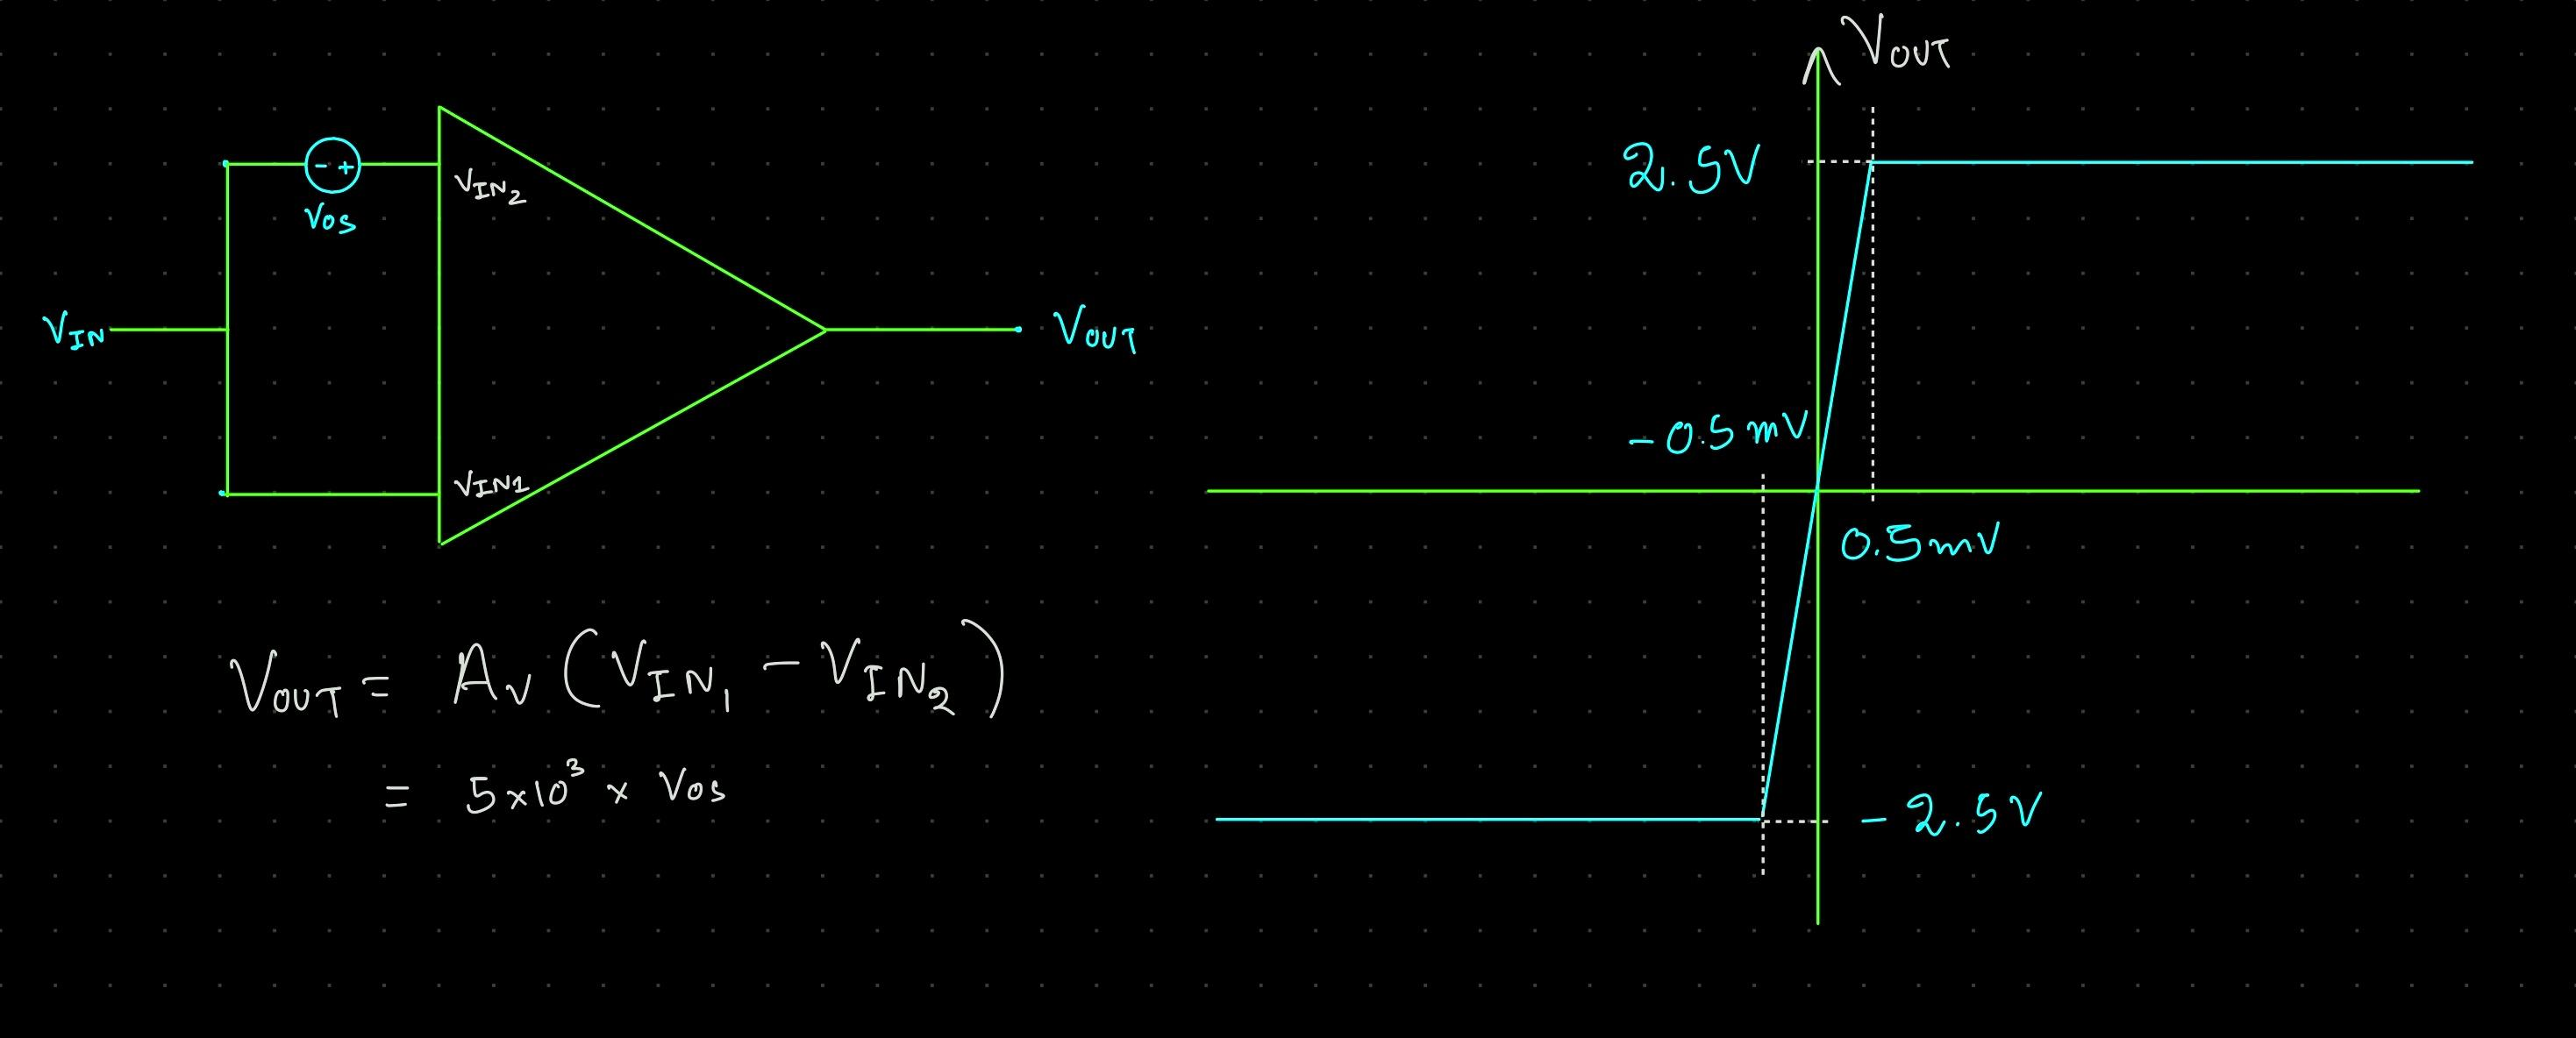
\includegraphics[keepaspectratio]{fig10.jpeg}}

}

\caption{Open-Loop gain with offset voltage shown externally}

\end{figure}%

To measure the open-loop gain, I have tried two different methods.

\subsubsection{The LC Method}\label{the-lc-method}

This is a conceptually neat method. A large inductor is used between the
feedback between \(V_{out}\) and \(V_{IN1}\), and a large capacitor is
used between \(V_{IN1}\) and \(GND\).

At DC level, \(f=0\), so the inductor acts as a short circuit, while the
capacitor acts as open circuit, this results in the amplifier working as
a unity gain amplifier.

When a small AC signal (say, \(V_{in})\) is applied, the inductor, which
has a large value, essentially operates as an open circuit, while the
capacitor acts as a short circuit to \(GND\). So,
\(V_{out} = A_{v}.V_{in}\).

The test bench and simulation results with this method are given in Fig
11 and Fig 12.

\pandocbounded{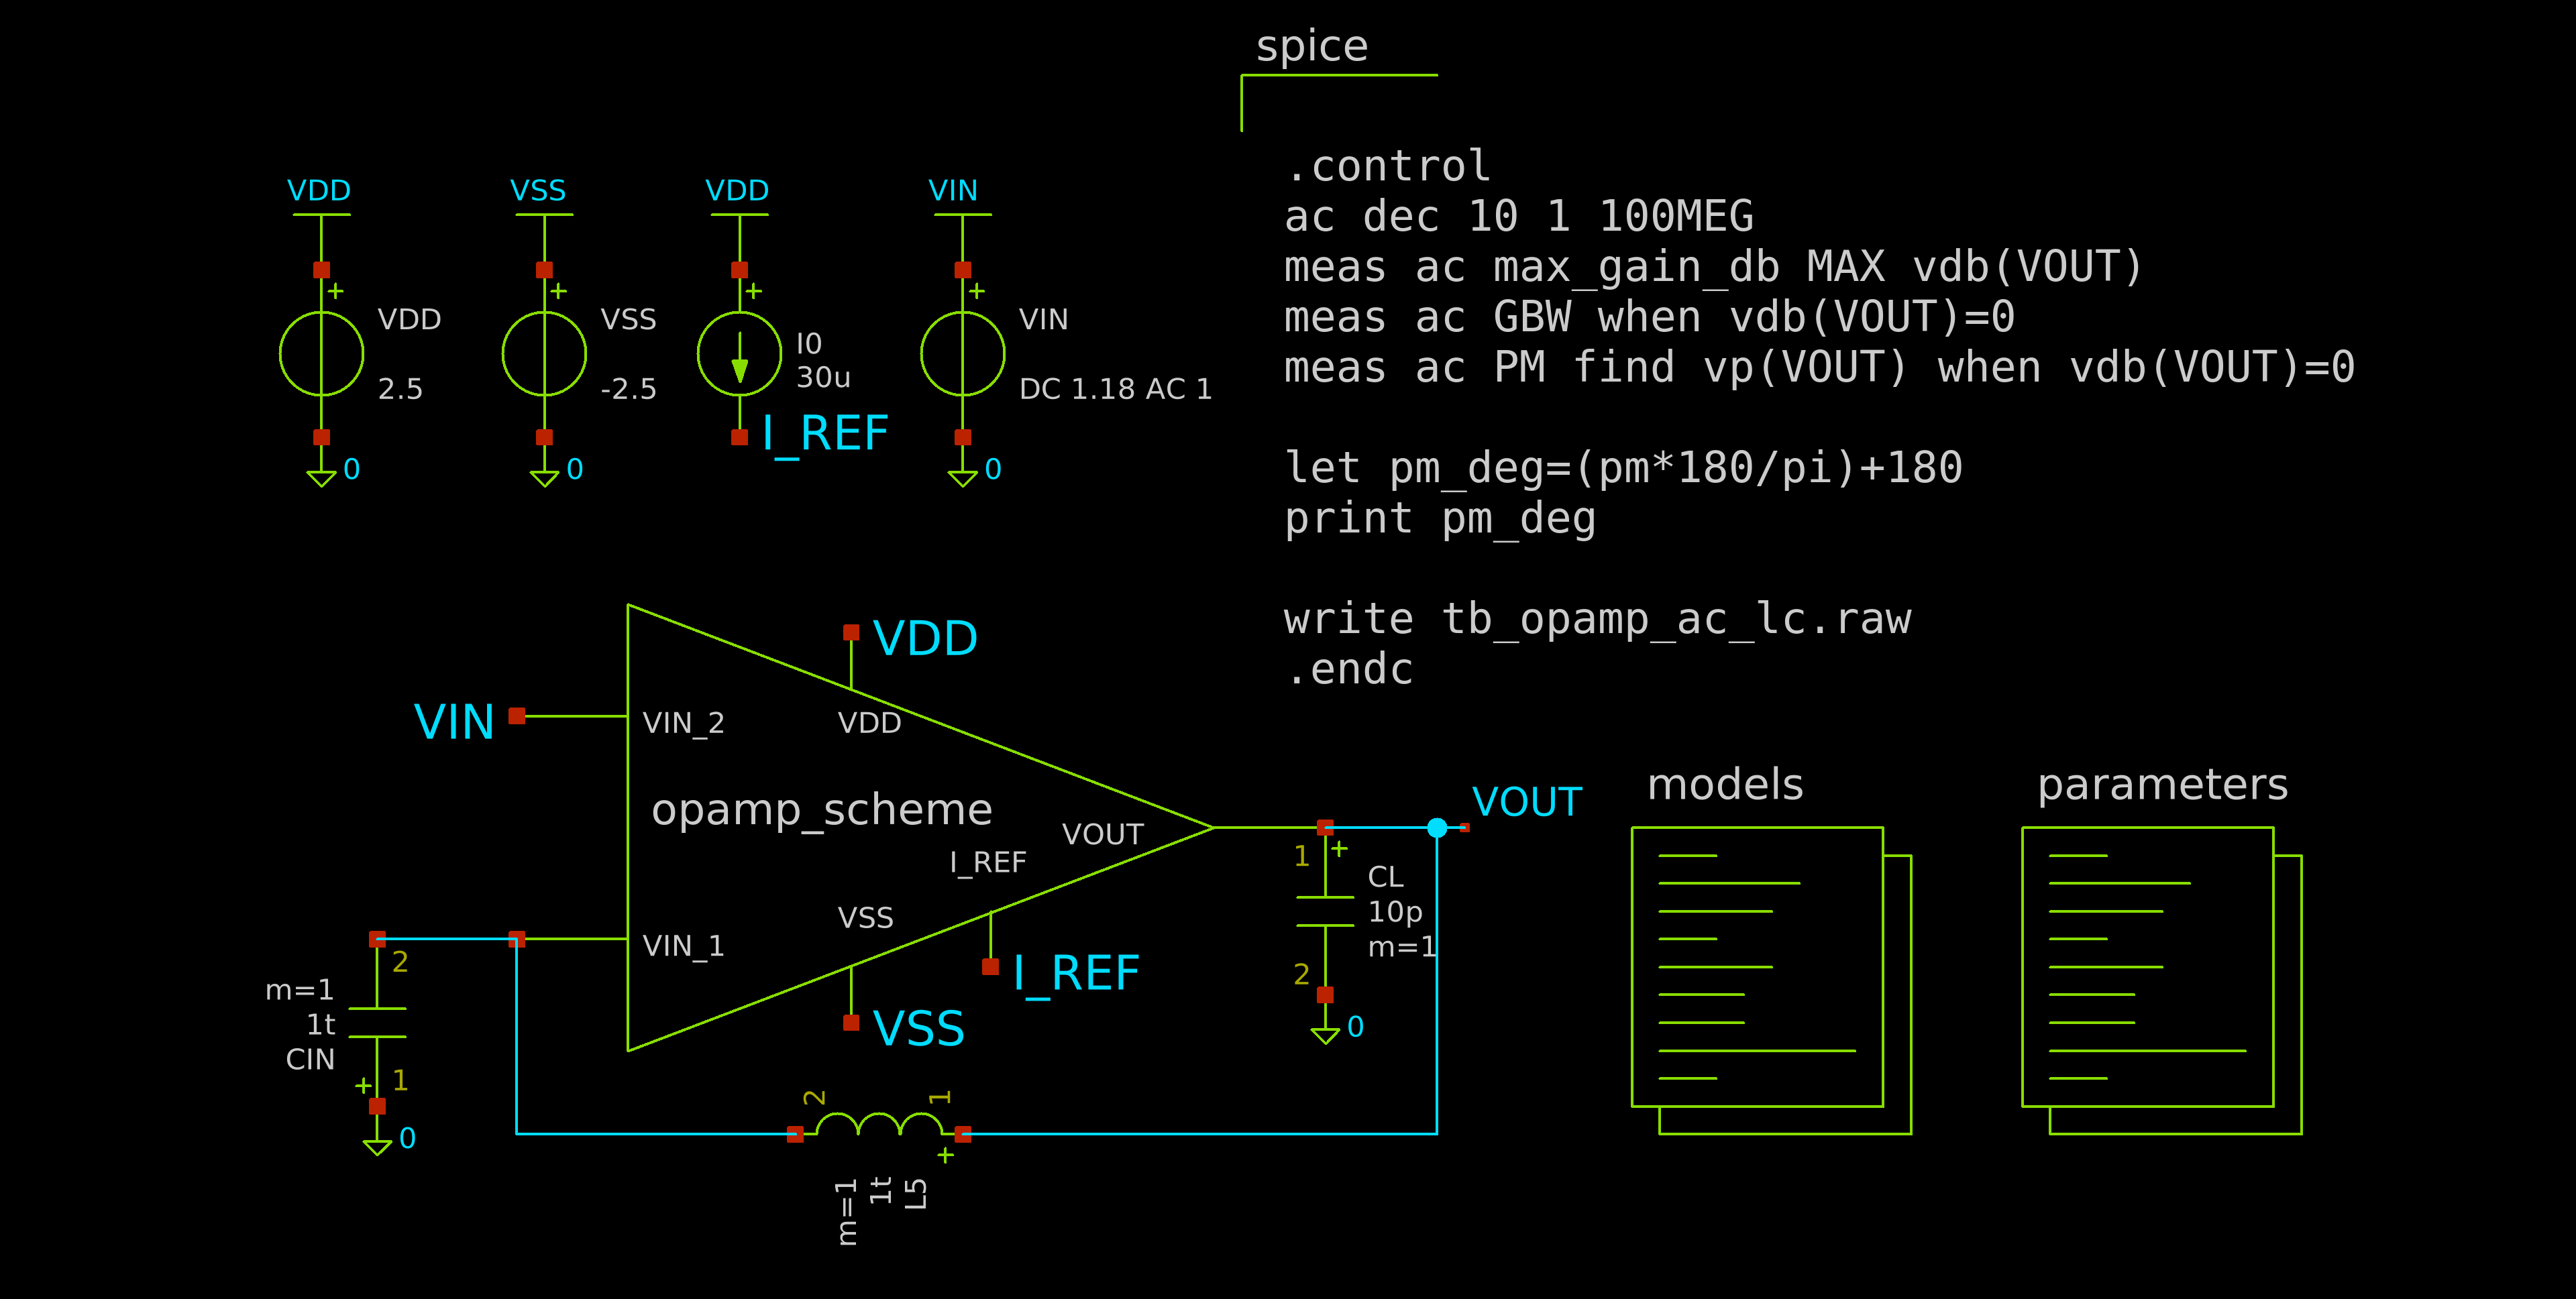
\includegraphics[keepaspectratio,alt={Test Bench}]{tb_opamp_ac_lc.png}}
\pandocbounded{\includegraphics[keepaspectratio,alt={Bode Plot}]{res_opamp_ac_lc.png}}

However, this is not a practical method, since such large inductors and
capacitors are generally not available.

\subsubsection{The RC Method}\label{the-rc-method}

This method uses a large resistor \((R_f)\) in place of the inductor.
Because the gate terminal of the input MOSFET has very high DC
impedance, the steady-state current flowing through the feedback loop is
approximately zero (\(I_f \approx 0\)). Consequently, there is zero
voltage drop across \(R_f\), this forces \(V_{out} = V_{in1}\) and
causes the circuit to operate as a unity-gain amplifier at DC.

On applying a small AC signal, the capacitor acts as a short-circuit to
\(GND\). So, again operating in the open-loop configuration,
\(V_{out} = A_{v}.V_{in}\).

In this circuit, it is necessary to select the \(\frac{1}{RC}\) time
constant a factor of \(A_v(0)\) less than the anticipated dominant pole
of the op-amp. The true open loop characteristics will not be observed
until the frequency is approximately \(\frac{A_v(0)}{RC}\), Above this
frequency, the gain is essentially the open-loop gain of the op-amp.
This method works well for both simulation and measurement.

\paragraph{Component Selection}\label{component-selection}

To make sure the newly introduced zero doesn't interfere with our gain,
values of \(C_{in} = 10uF\) and \(R_f = 10M\Omega\) were chosen so the
pole lies very close to the origin.

\(f_{z} = \frac{1}{2.\pi.RC} \approx 1.59mHz\)

As mentioned above, the true open loop characteristics will not be
observed until the frequency is approximately \(\frac{A_v(0)}{RC}\),
i.e, the new pole.

\(f_{obs} = \frac{A_{v}(0)}{2.\pi.RC} \approx 8.9Hz\)

So, we begin seeing the open-loop gain near 10Hz.

The test bench and simulation results with this method are given in Fig
13 and Fig 14.

\pandocbounded{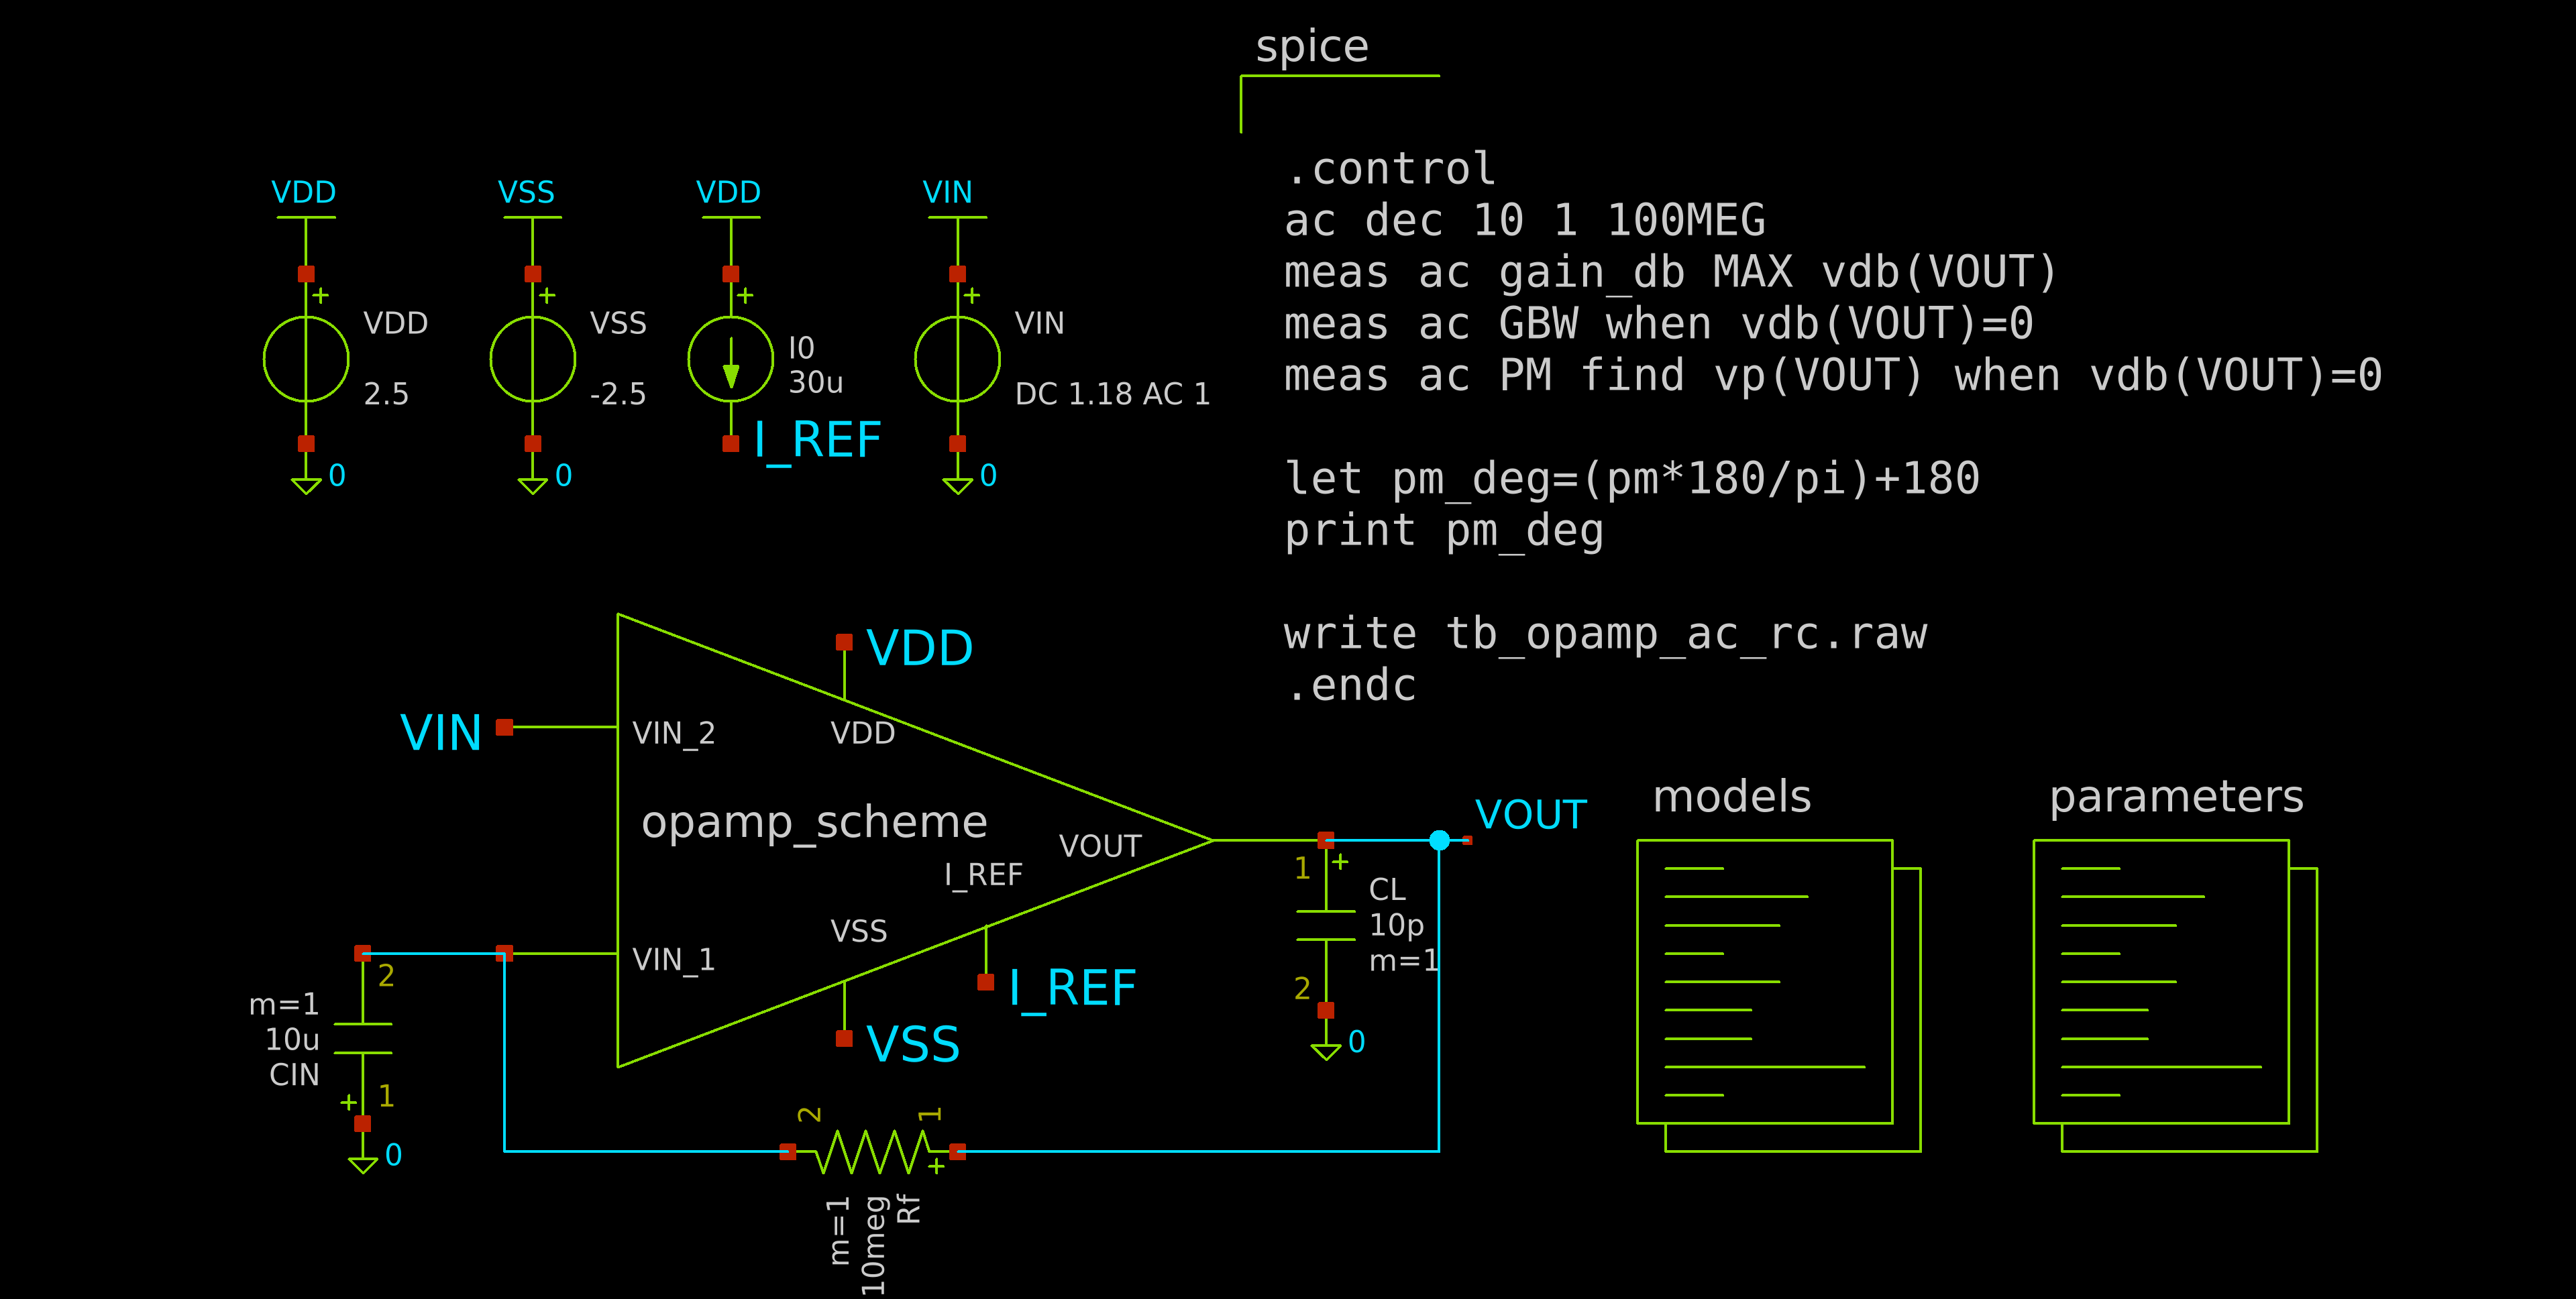
\includegraphics[keepaspectratio,alt={Test Bench}]{tb_opamp_ac_rc.png}}
\pandocbounded{\includegraphics[keepaspectratio,alt={Bode Plot}]{res_opamp_ac_rc.png}}

The results using both methods are given below:

{\def\LTcaptype{none} % do not increment counter
\begin{longtable}[]{@{}llll@{}}
\toprule\noalign{}
Parameter & LC Method & RC Method & Specification \\
\midrule\noalign{}
\endhead
\bottomrule\noalign{}
\endlastfoot
Max Gain & 74.07 dB & 74.00 dB & \textgreater73.98 dB \\
GBW & 5.85 MHz & 5.85 MHz & 5 MHz \\
Phase Margin & 63.18° & 63.19 & \textgreater60° \\
\end{longtable}
}

\subsection{Transient Response and Slew
Rate}\label{transient-response-and-slew-rate}

A large-signal step input was applied to measure the slew rate. The test
bench and output waveforms are shown in Fig 15 and Fig 16.

\pandocbounded{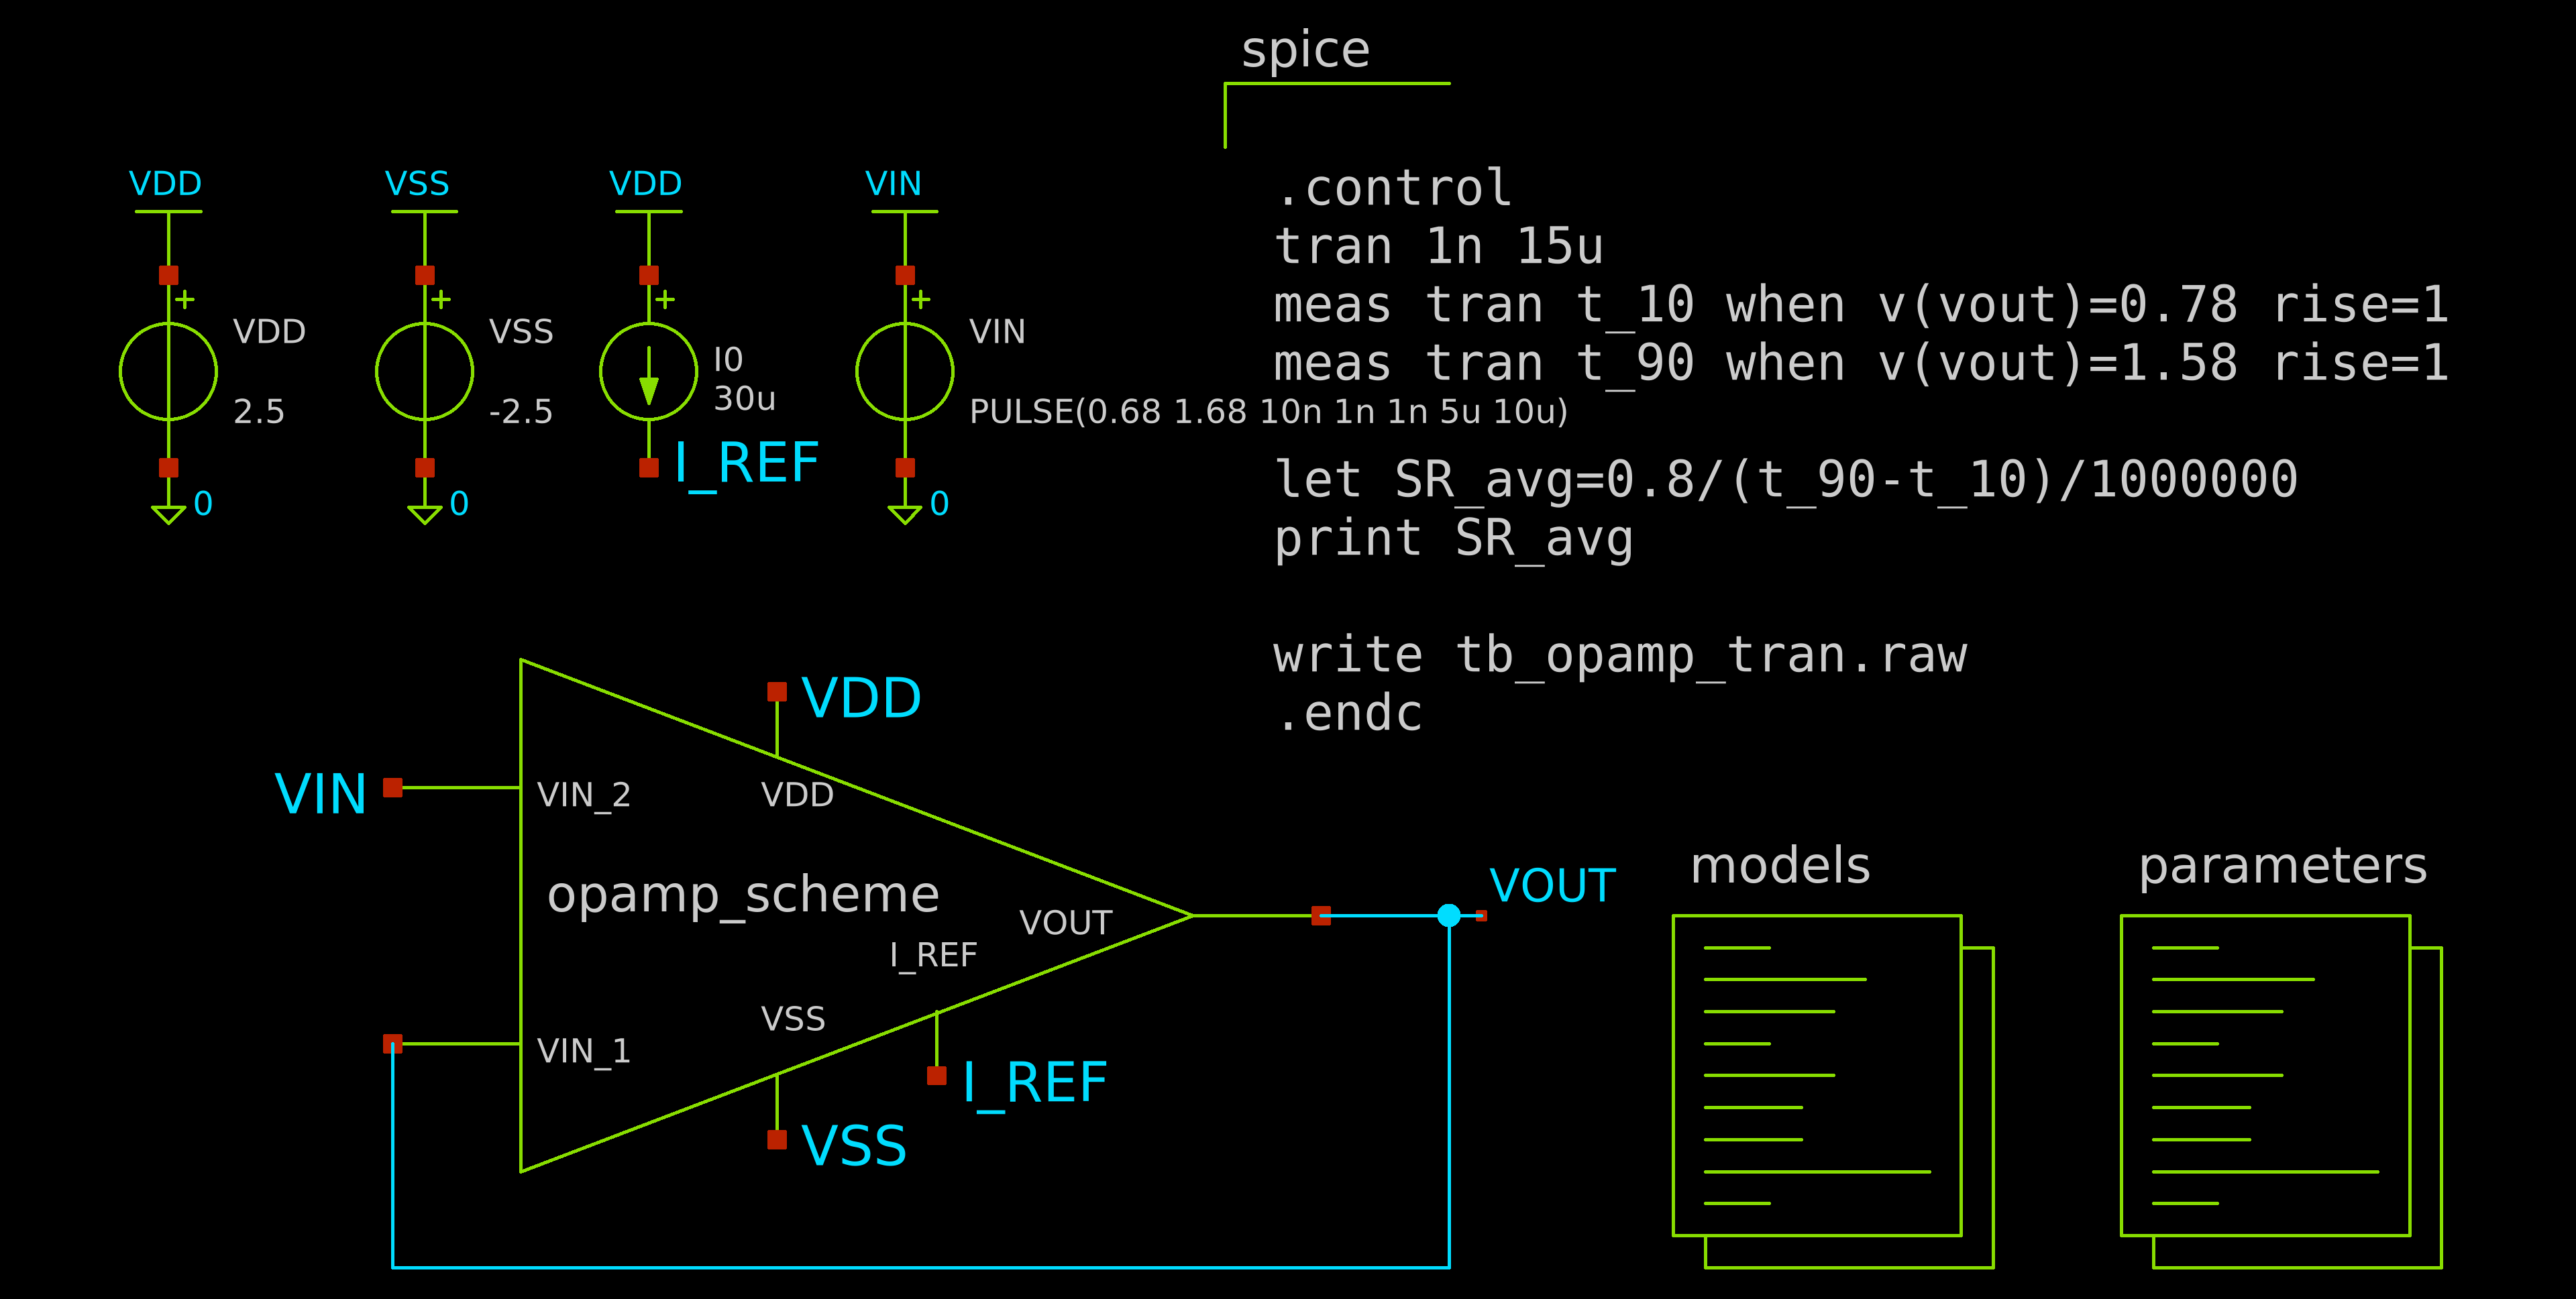
\includegraphics[keepaspectratio,alt={Test Bench}]{tb_opamp_tran.png}}
\pandocbounded{\includegraphics[keepaspectratio,alt={Tran PLot}]{res_opamp_tran.png}}

The average slew rate is measured between 10\% and 90\% of the final
voltage swing. It is found to be:

\(SR = 10.637V/{\mu}s\)

\subsection{DC Sweep - Linear Output
Swing}\label{dc-sweep---linear-output-swing}

The linear output swing is defined as the voltage range over which the
amplifier maintains at least 90\% of its ideal gain. Because the circuit
is configured as a unity-gain buffer, the ideal DC transfer
characteristic has a slope of \(1\space{V/V}\). Therefore, the absolute
limits of the output swing are identified as the points where the
derivative of the transfer curve \(\frac{dV_{out}}{dV_{in}}\) drops
below \(0.9 \space V/V\)

The test bench and simulation result are given in Fig 17 and Fig 18.

\pandocbounded{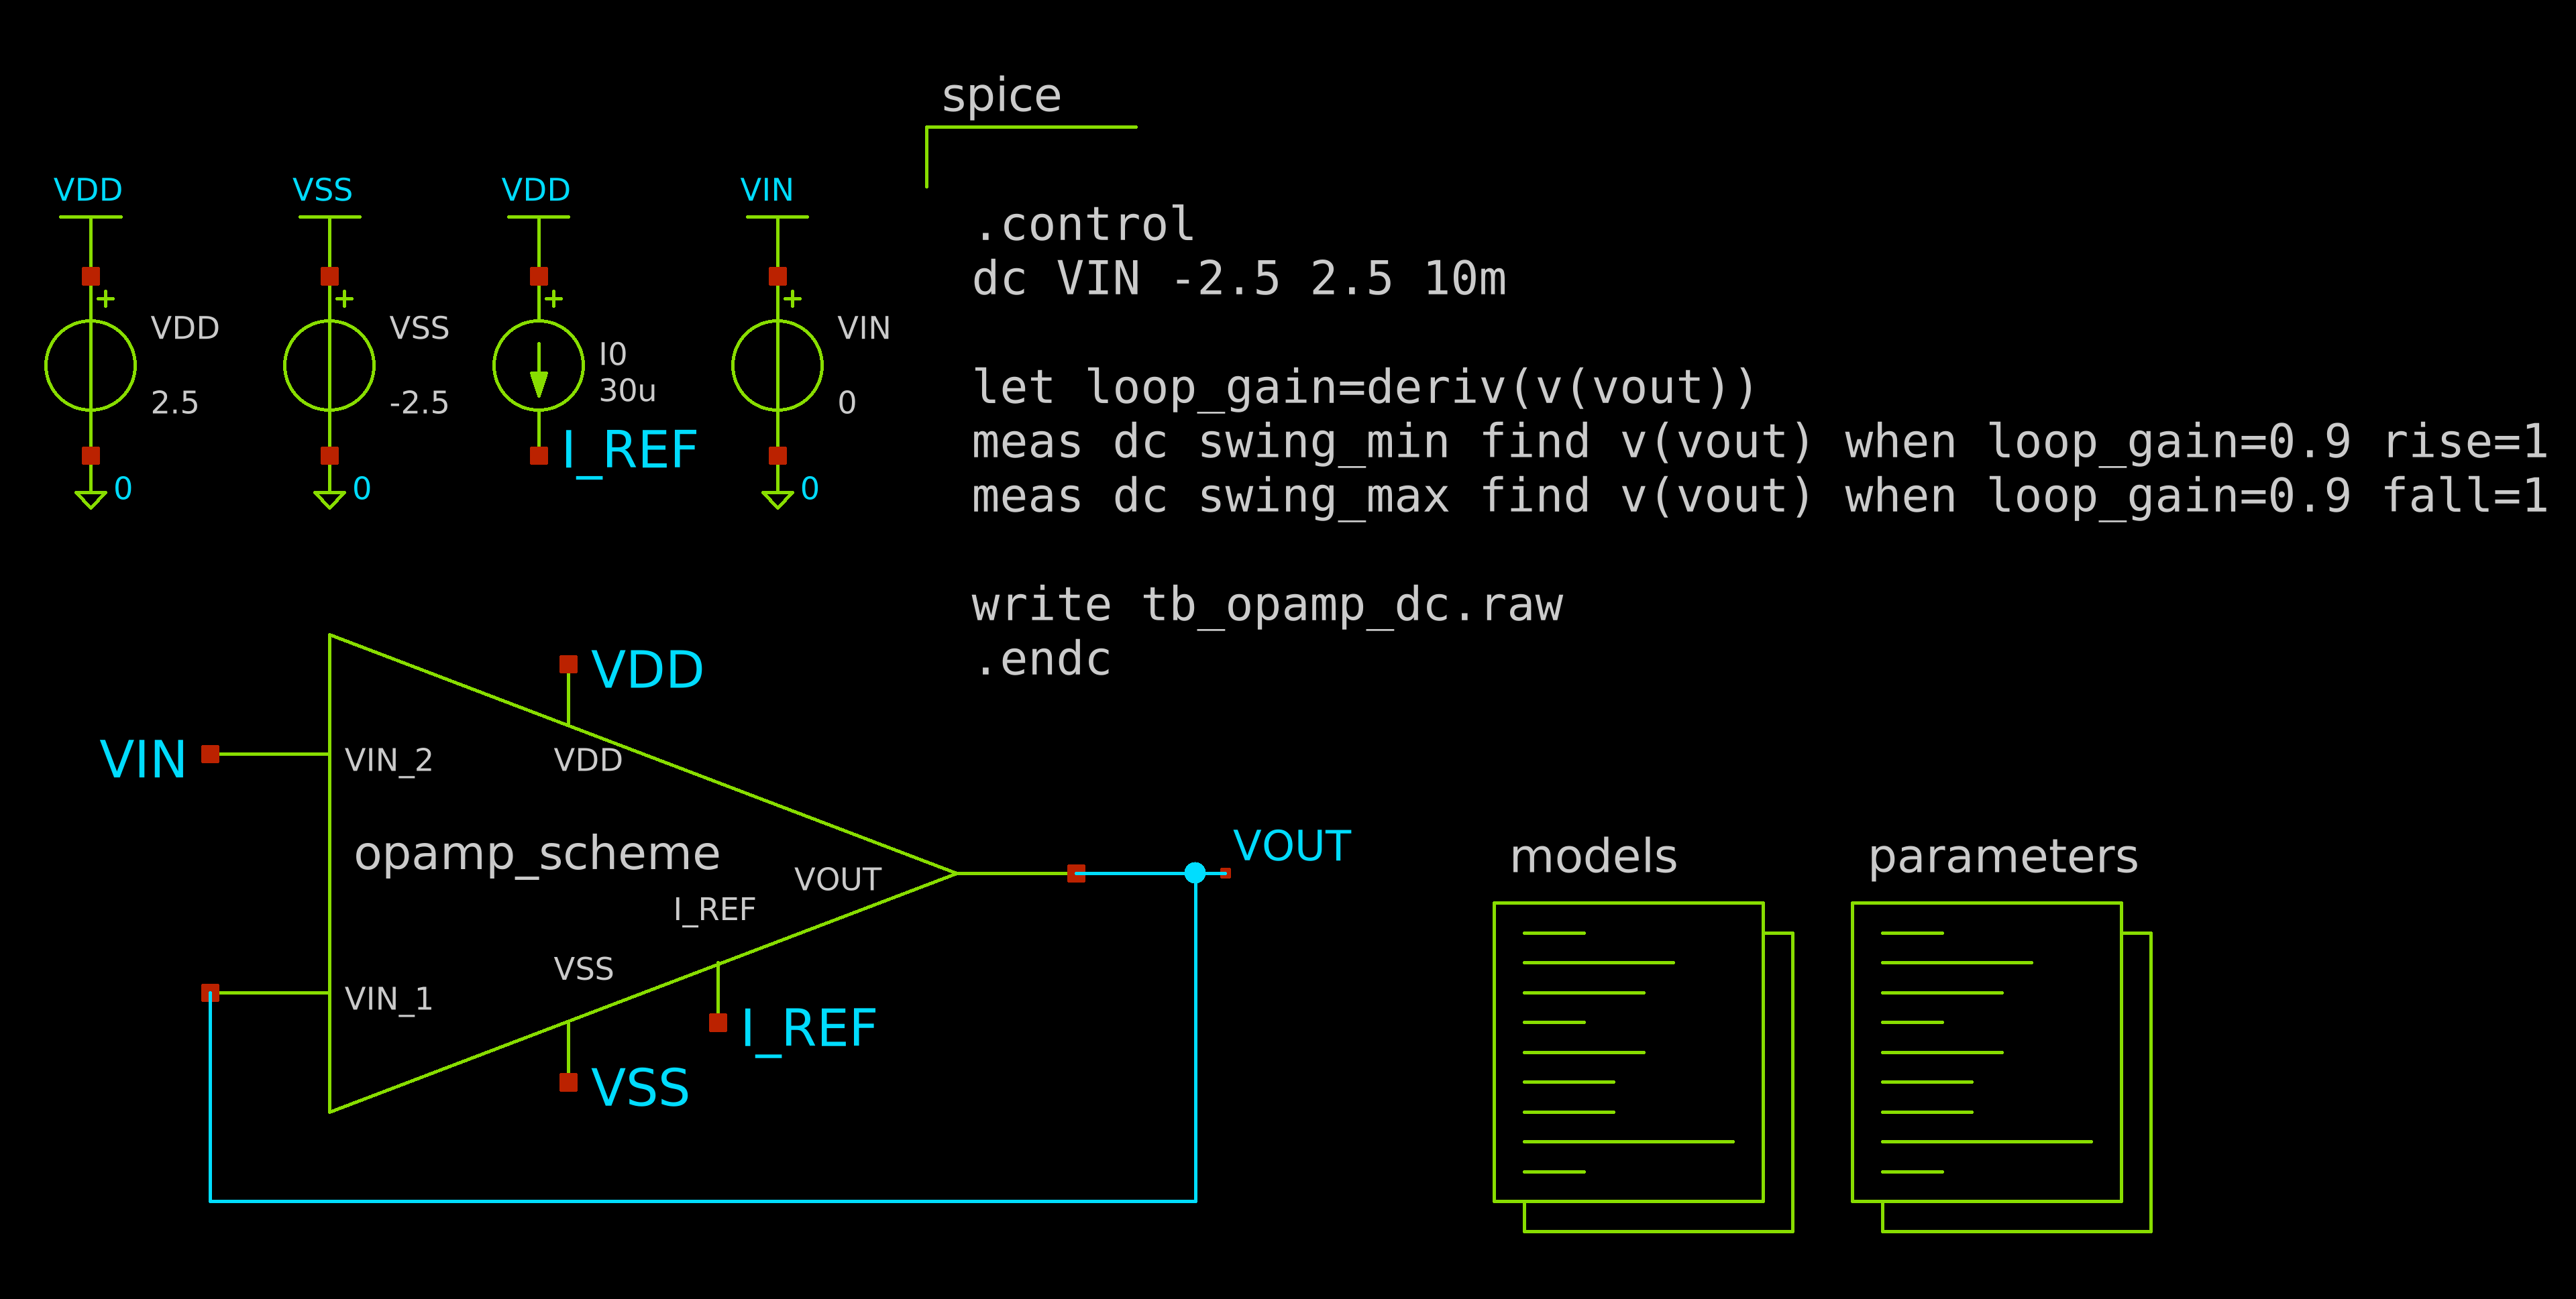
\includegraphics[keepaspectratio,alt={Test Bench}]{tb_opamp_dc.png}}
\pandocbounded{\includegraphics[keepaspectratio,alt={DC Plot}]{res_opamp_dc.png}}

The results obtained are given below:

\begin{itemize}
\tightlist
\item
  \(V_{out}(max) = 2.44V\)
\item
  \(V_{out}(min) = -2.27V\)
\end{itemize}

\begin{center}\rule{0.5\linewidth}{0.5pt}\end{center}

\section{Design Iterations}\label{design-iterations}

\subsection{\texorpdfstring{Iteration 1 - Initial Sizing
(\(\frac{W}{L} = 3\) for M1 and
M2)}{Iteration 1 - Initial Sizing (\textbackslash frac\{W\}\{L\} = 3 for M1 and M2)}}\label{iteration-1---initial-sizing-fracwl-3-for-m1-and-m2}

{\def\LTcaptype{none} % do not increment counter
\begin{longtable}[]{@{}lll@{}}
\toprule\noalign{}
Parameter & Target & Result \\
\midrule\noalign{}
\endhead
\bottomrule\noalign{}
\endlastfoot
Max Gain & \(> 73.98 dB\) & \(73.25 dB\) \\
GBW & \(5 MHz\) & \(4.55 MHz\) \\
Phase Margin & \(>60^{\circ}\) & \(68.08^{\circ}\) \\
\end{longtable}
}

Both Max Gain and GBW were not upto specification.

Since \(GBW = \frac{g_{m1}}{2\pi C_c}\) and
\(g_{m1} = \sqrt{2K'_p \cdot \frac{W}{L} \cdot I_{D1}}\), increasing
\(g_{m1}\) simultaneously increases both GBW as well as the first-stage
gain.

So, increasing \(\frac{W}{L}\) for M1 and M2 may be the way to go.

\subsection{\texorpdfstring{Iteration 2 - (\(\frac{W}{L} = 3.5\) for M1
and
M2)}{Iteration 2 - (\textbackslash frac\{W\}\{L\} = 3.5 for M1 and M2)}}\label{iteration-2---fracwl-3.5-for-m1-and-m2}

{\def\LTcaptype{none} % do not increment counter
\begin{longtable}[]{@{}lll@{}}
\toprule\noalign{}
Parameter & Target & Result \\
\midrule\noalign{}
\endhead
\bottomrule\noalign{}
\endlastfoot
Max Gain & \(> 73.98 dB\) & \(74.07 dB\) \\
GBW & \(5 MHz\) & \(4.96 MHz\) \\
Phase Margin & \(>60^{\circ}\) & \(66.20^{\circ}\) \\
Slew Rate & \(>10V/{\mu}s\) & \(8.86V/{\mu}s\) \\
\end{longtable}
}

While the gain and GBW seem to be well within specifications, the slew
rate is lower than our target.

\$ SR = \frac{I_{5}}{C_{c}} \$, we may either try increasing \(I_5\) or
decreasing \(C_{c}\). Increasing \(I_5\) requires us to go through every
calculation step above again to get the updated sizing.

Our use of \(C_c = 3pF\) is well above the condition of
\(C_c > 0.22C_L\), which means \(C_c > 2.2pF\).

Let us choose \(C_c = 2.5pF\)

\subsection{\texorpdfstring{Iteration 3 -
(\(C_c = 2.5pF\))}{Iteration 3 - (C\_c = 2.5pF)}}\label{iteration-3---c_c-2.5pf}

{\def\LTcaptype{none} % do not increment counter
\begin{longtable}[]{@{}lll@{}}
\toprule\noalign{}
Parameter & Target & Result \\
\midrule\noalign{}
\endhead
\bottomrule\noalign{}
\endlastfoot
Max Gain & \(> 73.98 dB\) & \(74.07 dB\) \\
GBW & \(5 MHz\) & \(5.85 MHz\) \\
Phase Margin & \(>60^{\circ}\) & \(63.18^{\circ}\) \\
Slew Rate & \(>10V/{\mu}s\) & \(10.64V/{\mu}s\) \\
\end{longtable}
}

Now we seem to be within good margins of out specifications.

We will adopt this sizing.

\section{Final Performance Summary}\label{final-performance-summary}

{\def\LTcaptype{none} % do not increment counter
\begin{longtable}[]{@{}
  >{\raggedright\arraybackslash}p{(\linewidth - 4\tabcolsep) * \real{0.2000}}
  >{\raggedright\arraybackslash}p{(\linewidth - 4\tabcolsep) * \real{0.3286}}
  >{\raggedright\arraybackslash}p{(\linewidth - 4\tabcolsep) * \real{0.4714}}@{}}
\toprule\noalign{}
\begin{minipage}[b]{\linewidth}\raggedright
Parameter
\end{minipage} & \begin{minipage}[b]{\linewidth}\raggedright
Target
\end{minipage} & \begin{minipage}[b]{\linewidth}\raggedright
Result
\end{minipage} \\
\midrule\noalign{}
\endhead
\bottomrule\noalign{}
\endlastfoot
Max Gain & \(> 73.98 dB\) & \(74.07 dB\) \\
GBW & \(5 MHz\) & \(5.85 MHz\) \\
Phase Margin & \(>60^{\circ}\) & \(63.18^{\circ}\) \\
Slew Rate & \(> 10 \space V/\mu s\) & \(10.64 \space V/\mu s\) \\
Power & \(< 2mW\) & \(1.188mW\) \\
Output Swing & \(\pm 2V\) & \(-2.27 \space to \space 2.44 V\) \\
\end{longtable}
}

\subsection{The Transistor and Component values
used:}\label{the-transistor-and-component-values-used}

{\def\LTcaptype{none} % do not increment counter
\begin{longtable}[]{@{}llll@{}}
\toprule\noalign{}
Transistor & Type & W/L & Current \(({\mu}A)\) \\
\midrule\noalign{}
\endhead
\bottomrule\noalign{}
\endlastfoot
M1, M2 & NMOS & 3.5 & 15.45, 15.48 \\
M3, M4 & PMOS & 10 & 15.45, 15.48 \\
M5 & NMOS & 3 & 30.93 \\
M6 & PMOS & 86.6 & 176.68 \\
M7 & NMOS & 13 & 176.68 \\
M8 & NMOS & 3 & 30.00 \\
\end{longtable}
}

Component values: \(C_c = 2.5pF\), \(C_L = 10pF\)

\section{Limitations and Known
Critiques}\label{limitations-and-known-critiques}

The Miller-compensated two-stage OTA with a compensation capacitor has
known limitations. Jacob Baker notes in his resources that this
topology, particularly with a zero-nulling resistor, has practical
drawbacks compared to more modern compensation strategies.

\begin{figure}[H]

{\centering \pandocbounded{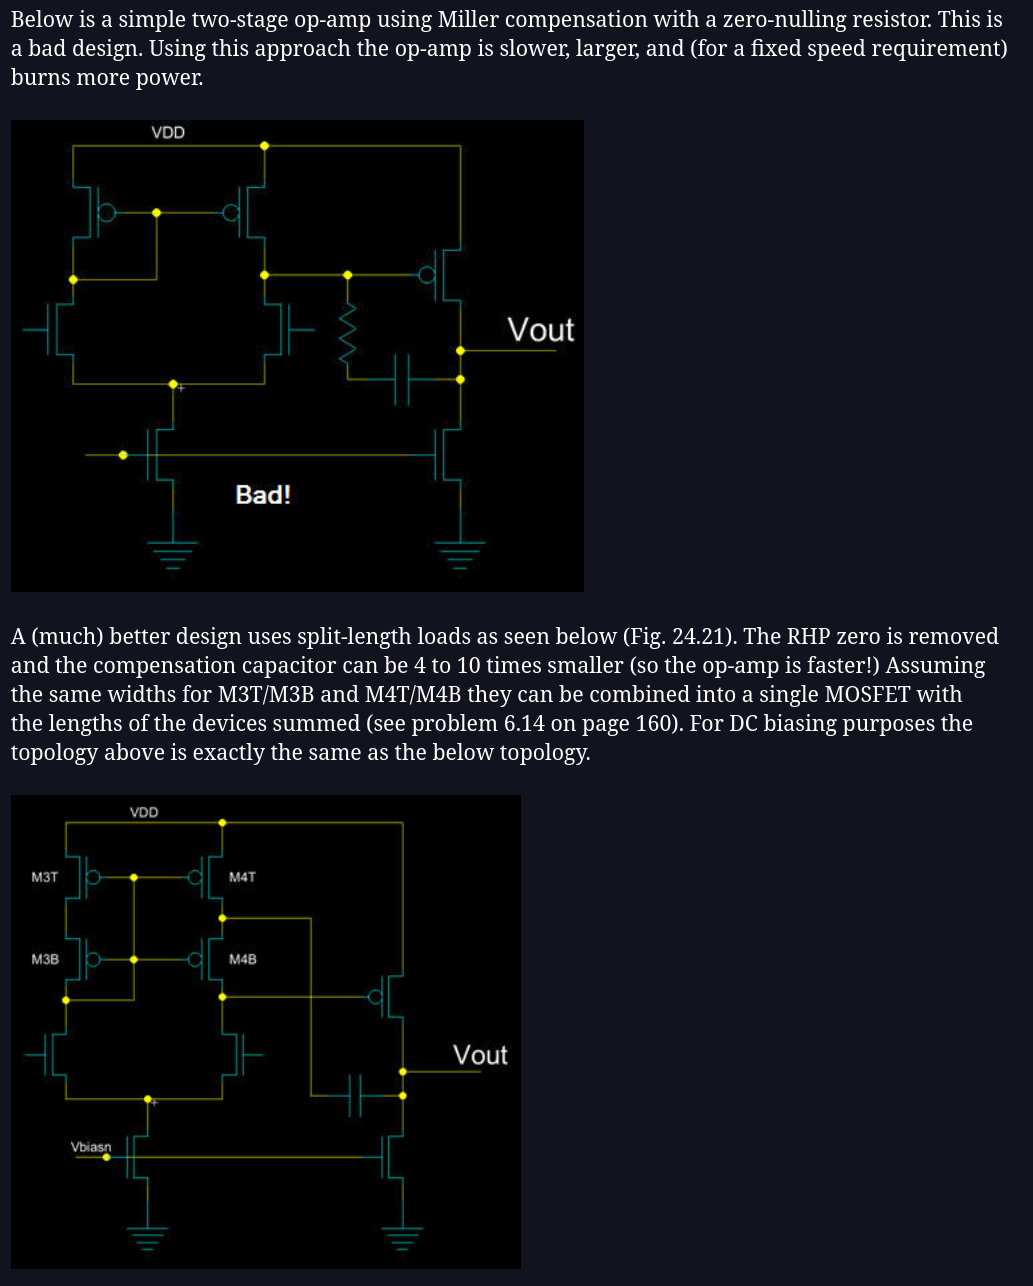
\includegraphics[keepaspectratio]{fig19.png}}

}

\caption{Baker's critique}

\end{figure}%

The goal of this project was to learn design methodology rather than
implement a production-ready topology. The two-stage Miller-compensated
OTA remains the standard introductory circuit for this purpose,
providing clear insight into compensation theory, pole-zero placement,
and the gain-bandwidth tradeoff. Exploring Baker's recommended
alternatives is a natural next step.

\section{References}\label{references}

\protect\phantomsection\label{refs}
\begin{CSLReferences}{1}{1}
\bibitem[\citeproctext]{ref-allen_cmos}
Allen, Phillip E., and Douglas R. Holberg. 2011. \emph{CMOS Analog
Circuit Design}. 3rd ed. Oxford University Press.

\end{CSLReferences}

\section{Personal Note}\label{personal-note}

In this document, I have tried to include everything I have learnt
designing this project as an absolute beginner to both SPICE as well as
analog electronics in general.

I have spent nearly a month on this topic, out of which only about a
week or two was spent on building this. I first discovered the two-stage
CMOS OTA in an IEEE conference paper by M. Kadam, which used skywater
pdk, I tried to understand it, but couldn't get an intuitive feel for
why the design choices were made the way they were. But this motivated
me to try design this, since it seemed to use the basic building blocks
I had already studied. I followed up with youtube videos on the same
topic, but again, while I was following the steps, I didn't understand
why we were making the choices that we were, but at the same time, I
felt I was getting somewhat more comfortable with the topic. I followed
up with
\href{https://www.reddit.com/r/chipdesign/comments/1t0mj9j/how_do_you_actually_design_a_circuit/}{this
question on Reddit} and got incredibly helpful and detailed answers.
Specifically, user u/Fast\_Document1643 was very helpful, replied to all
my questions with great patience, even if they were basic, and also
pointed me towards the book I used as my main source of reference here:
CMOS Analog Circuit Design by Allen \& Holberg.\\
Anyway, this went through the entire process of the design and the steps
followed here are taken from the book.

I was also stuck in measuring the operating points and open loop gain
for a long time, scratching my head cause my op-amp would just stick to
a value near the power supply. Like in every course, I have read that
the offset voltage getting multiplied with a huge gain causes this, but
I just couldn't think of that in my design process (I guess this is what
experience develops?). After realising this, work was a lot easier.

On the topic of other measurements, while I did know the concept of slew
rate and output voltage swing, I didn't know how to measure their exact
values, so I had to study up measurement techniques before actually
using the .dc or .tran commands to find them.

For iterations, I had surprisingly little to worry about. Allen \&
Holberg's book mentioned the exact pitfalls and exactly which values to
look into, so all I had to was mess with them and look at parameters
that were dependent on them and make sure all were within range. I
probably should have rounded up the \(\frac{W}{L}\) ratio of M6 to 87
instead of keeping it at 86.6, but I kinda forgot I didn't until
everything was done, and when all the parameters seemed be within
margin, I didn't really want to change anything.




\end{document}
